%----------------------------------------------------------------------------------------
%	PACKAGES AND OTHER DOCUMENT CONFIGURATIONS
%----------------------------------------------------------------------------------------

\documentclass[14pt]{article} % Document font size and equations flushed left

\usepackage[english]{babel} % Specify a different language here - english by default

% \usepackage{lipsum} % Required to insert dummy text. To be removed otherwise

\usepackage{color}

%\usepackage{multicol}

\usepackage[margin=0.6in]{geometry}

% This package is for figures
\usepackage{graphicx}

%This package is to put an image inside the title:
\usepackage{titling}

%This package is for line breaks and new lines:
\usepackage[utf8]{inputenc}

%For hyperlinks:
\usepackage{hyperref}

\usepackage{float}

%The mathematical package:
%\usepackage{mathtools}

%to allow block commenting
\long\def\/*#1*/{}

\usepackage{textcomp}


%----------------------------------------------------------------------------------------
%	COLUMNS
%----------------------------------------------------------------------------------------

\setlength{\columnsep}{0.6cm} % Distance between the two columns of text
%\setlength{\fboxrule}{0.90pt} % Width of the border around the abstract

%----------------------------------------------------------------------------------------
%	COLORS
%----------------------------------------------------------------------------------------

\definecolor{red}{RGB}{100,0,0} 
\definecolor{blue}{RGB}{10,0,100} 
\definecolor{green}{RGB}{0,100,0} 
\definecolor{orange}{RGB}{110,60,40}


%----------------------------------------------------------------------------------------
%	ARTICLE INFORMATION
%----------------------------------------------------------------------------------------

\pretitle{%
  \begin{center}
  \LARGE
  
\includegraphics[height=5cm]{eusa-logo.jpg}\\[\bigskipamount]
}
\posttitle{\end{center}}

\title{\huge {\textbf{Basic Tech Training}}} % Article title

%\author{Martin, Cat, Louis, Rich and the rest} 
\date{March, 2017}




%----------------------------------------------------------------------------------------

\begin{document}
%\twocolumn[
\begin{@twocolumnfalse}
\maketitle

%\flushbottom % Makes all text pages the same height

\abstract{
This is the handout for the \textbf{Basic Tech Training}. It contains several important concepts that will help you to form/extend a solid technical knowledge basis. \\ 
}
 \end{@twocolumnfalse}


\section{Introduction}
\label{intro}
In the \textbf{Edinburgh University Students' Association} we take pride in the fact that our emplyees are capable of dealing effectively with technical problems, stressful situations and deadlines, while maintaining a positive "can-do" attitude.
The Basic Tech Training is thus aimed at helping you to form a strong basis of technical knowledge. It examines several important concepts and goes over important skills that are required for you to be a successful technician in this company. You will gain basic knowledge of electricity, sound systems, lighting systems and AV systems. We shall also look over fault finding and troubleshooting for each of the aforementioned systems.


\section{Power}
\label{power}

Let us start from the beginning. Every piece of technical equipment needs electricity to function. Today we take electricity for granted, but often we are unaware of exactly how it works. Here we shall take a look at a simplified description of this physical phenomenon. 

\subsection{Electricity}
\label{electricity}
One often hears the words “current”, “voltage” and “resistance”. It is very important to understand these three concepts well. Here we will look at a very brief explanation of them. If you want to learn things in more detail, take a look at the following resources: \href{https://www.howequipmentworks.com/electricity_basics/}{howequipmentworks.com} and \href{https://en.wikipedia.org/wiki/Electricity#Electric_charge}{wikipedia.org}.

It is important that you know about electricity. It will help you to better understand electrical safety. Here we describe some of the basic principles of electricity:

\begin{itemize}

\item Current is related to the flow of electrons and is measured in Amperes.

\item Potential difference is what makes the electrons flow (current) and is measured in “Volts”. There are many sources of potential difference such as batteries, electrical supply sockets at home and hospital etc. Current is directly related to the potential difference, and this forms part of Ohms Law.

\item Resistance is something that resists current flow and is measured in Ohms. Current is inversely proportional to resistance. This relationship forms part of Ohms Law.

\item Ohms Law (\textbf{$V = I R$}) defines the relationship between \textit{voltage (V)}, \textit{current (I)}, and \textit{resistance (R)}. If you know two of the three components of Ohms Law, you can find out the third.

\item Current can be DC (Direct) or AC (Alternating). In DC, the electrons flow in one direction whereas in AC, the electrons alternate their direction.

\item Transformers are needed to make high voltages needed to economically send current over long distances. Transformers work only with AC, and that is why the power company supplies your home and hospital with AC.

\end{itemize}

\subsection{Electrical Cables}
\label{electrical-cables}
There are numerous different types of electrical cables. What is common for all of them is that they are used to provide \textbf{electrical power}. \textbf{Electrical power} is the rate, per unit time, at which electrical energy is transferred by an electric circuit (which includes cables). Now that we know what \textit{voltage (V)} and \textit{current (I)} are we can express \textit{power (P)} with the formula: \textbf{$P = I V$}. The SI unit of power is the \textbf{watt}. 

The plugs of electrical cables usually are defined by what current they can carry - 13 Amperes, 15 Amperes, 16 Amperes, etc. Thus, referring to the power formula, a cable plug with higher Amper classification can transfer more electrical power. This is important as for more powerful electrical equipment, you need to provide a suitable cable, otherwise \textbf{it will melt}.

Since we are in the UK we shall only look at the UK standard cable plugs. In the \textbf{Students' Association} you will most commonly encounter the following electrical cable plugs:

\begin{itemize}

\item 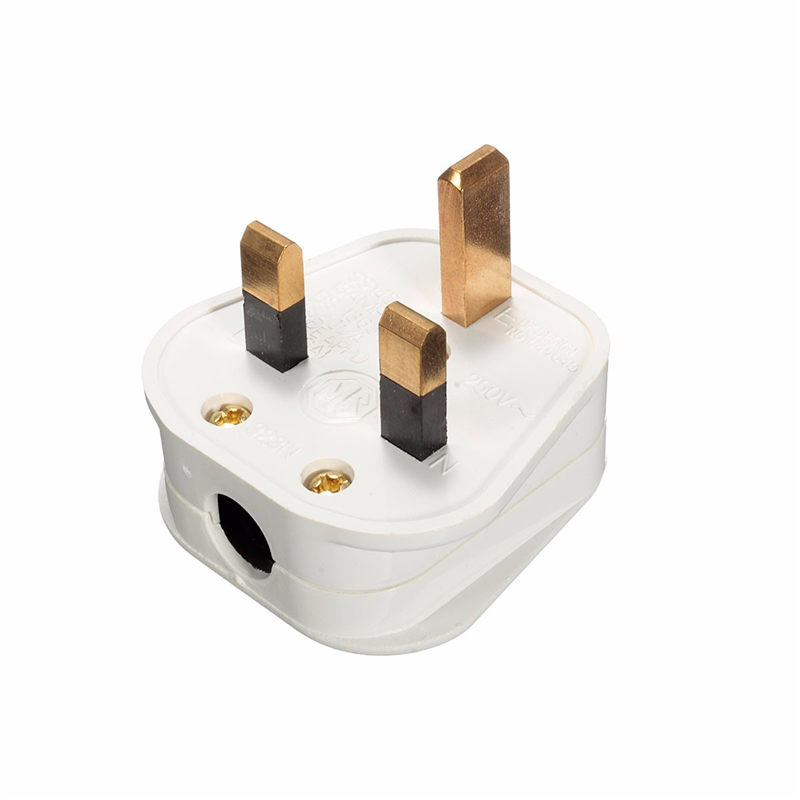
\includegraphics[scale=0.19]{13amp.jpg}\textbf{13 Amp:} This is your standard plug that you use to power laptops, desk lamps, iPhone chargers. In the Students' Association we use it to provide power on stage, charge laptops during conferences as well as to get power to our sound and lighting desks, projectors, etc.  

\item 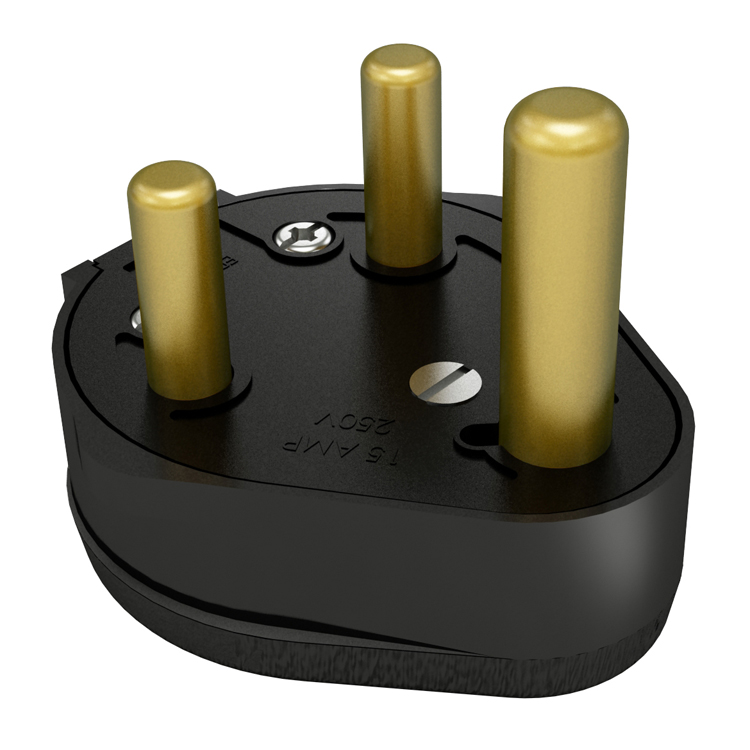
\includegraphics[scale=0.15]{15amp.jpg}\textbf{15 Amp:} This cable is almost exclusively used to power generic lights on a lighting rig. More detail is provided in the \textbf{Lighting Training}. 

\item 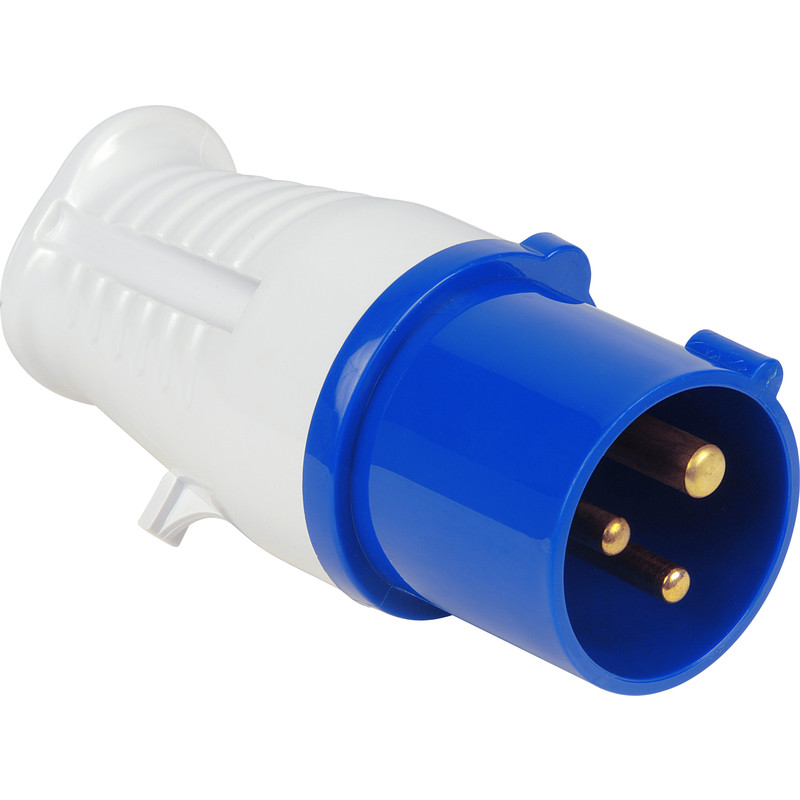
\includegraphics[scale=0.16]{16amp.jpg}\textbf{16 Amp:} This cable is widely used for different applications that require more power that what a 13 Amp supply can provide. The 16 Amp plug, unlike the 13 Amp one, can be used to provide power in an outside environment as it is waterproof. 

\item 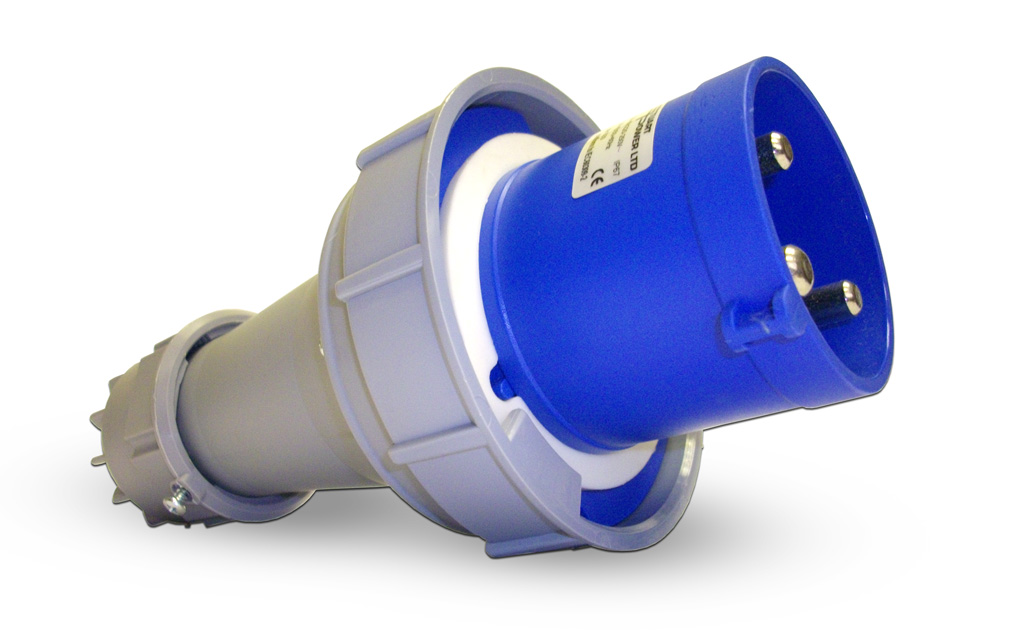
\includegraphics[scale=0.16]{32amp.jpg}\textbf{32 Amp:} This is a huge power plug that is used to provide even more power. They are often plugged into \textbf{Power Distribution Boxes}, which have multiple 16 Amp sockets. 

\item 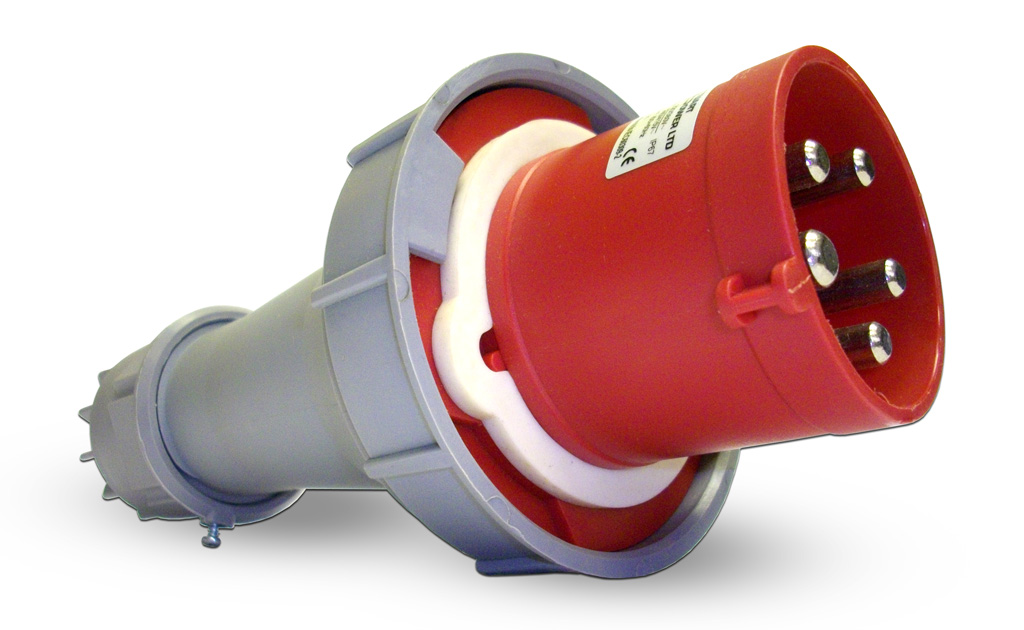
\includegraphics[scale=0.16]{63amp.jpg}\textbf{63 Amp:} Similar to 32 Amp, but larger in size and can provide even more power.

\end{itemize}


\section{Introduction to Sound and Audio Systems}
\label{intro-sound}
In physics, \textbf{sound} is a vibration that propagates as a typically audible mechanical wave of pressure and displacement, through a transmission medium such as air or water. Humans can hear sound waves with frequencies \textbf{between about 20 Hz and 20 kHz}. Sound above 20 kHz is called \textbf{ultrasound} and below 20 Hz is called \textbf{infrasound}.

Sound by itself can be very loud. If you do not believe that, visit a kindergarden at lunch break. However, it is often not loud enough. To help mitigate this problem we use a \textbf{Sound Reinforcement System}. 

\subsection{Structure of a Sound Reinforcement System}
\label{sound-system-structure}
A \textbf{Sound Reinforcement System} is the combination of microphones, signal processors, amplifiers, and loudspeakers in speaker cabinets that makes live or pre-recorded sounds louder and may also distribute those sounds to a larger or more distant audience. Such systems can range from very basic setups with a single microphone and/or music source up to massive line array systems with digital mixing desks and dozens of inputs. In general, though, the same principles apply to all of these systems, which helps to simplify them. A diagram of a typical sound reinforcement system is presented on Figure \ref{fig:intro}.

\begin{figure*}[h]
\begin{center}

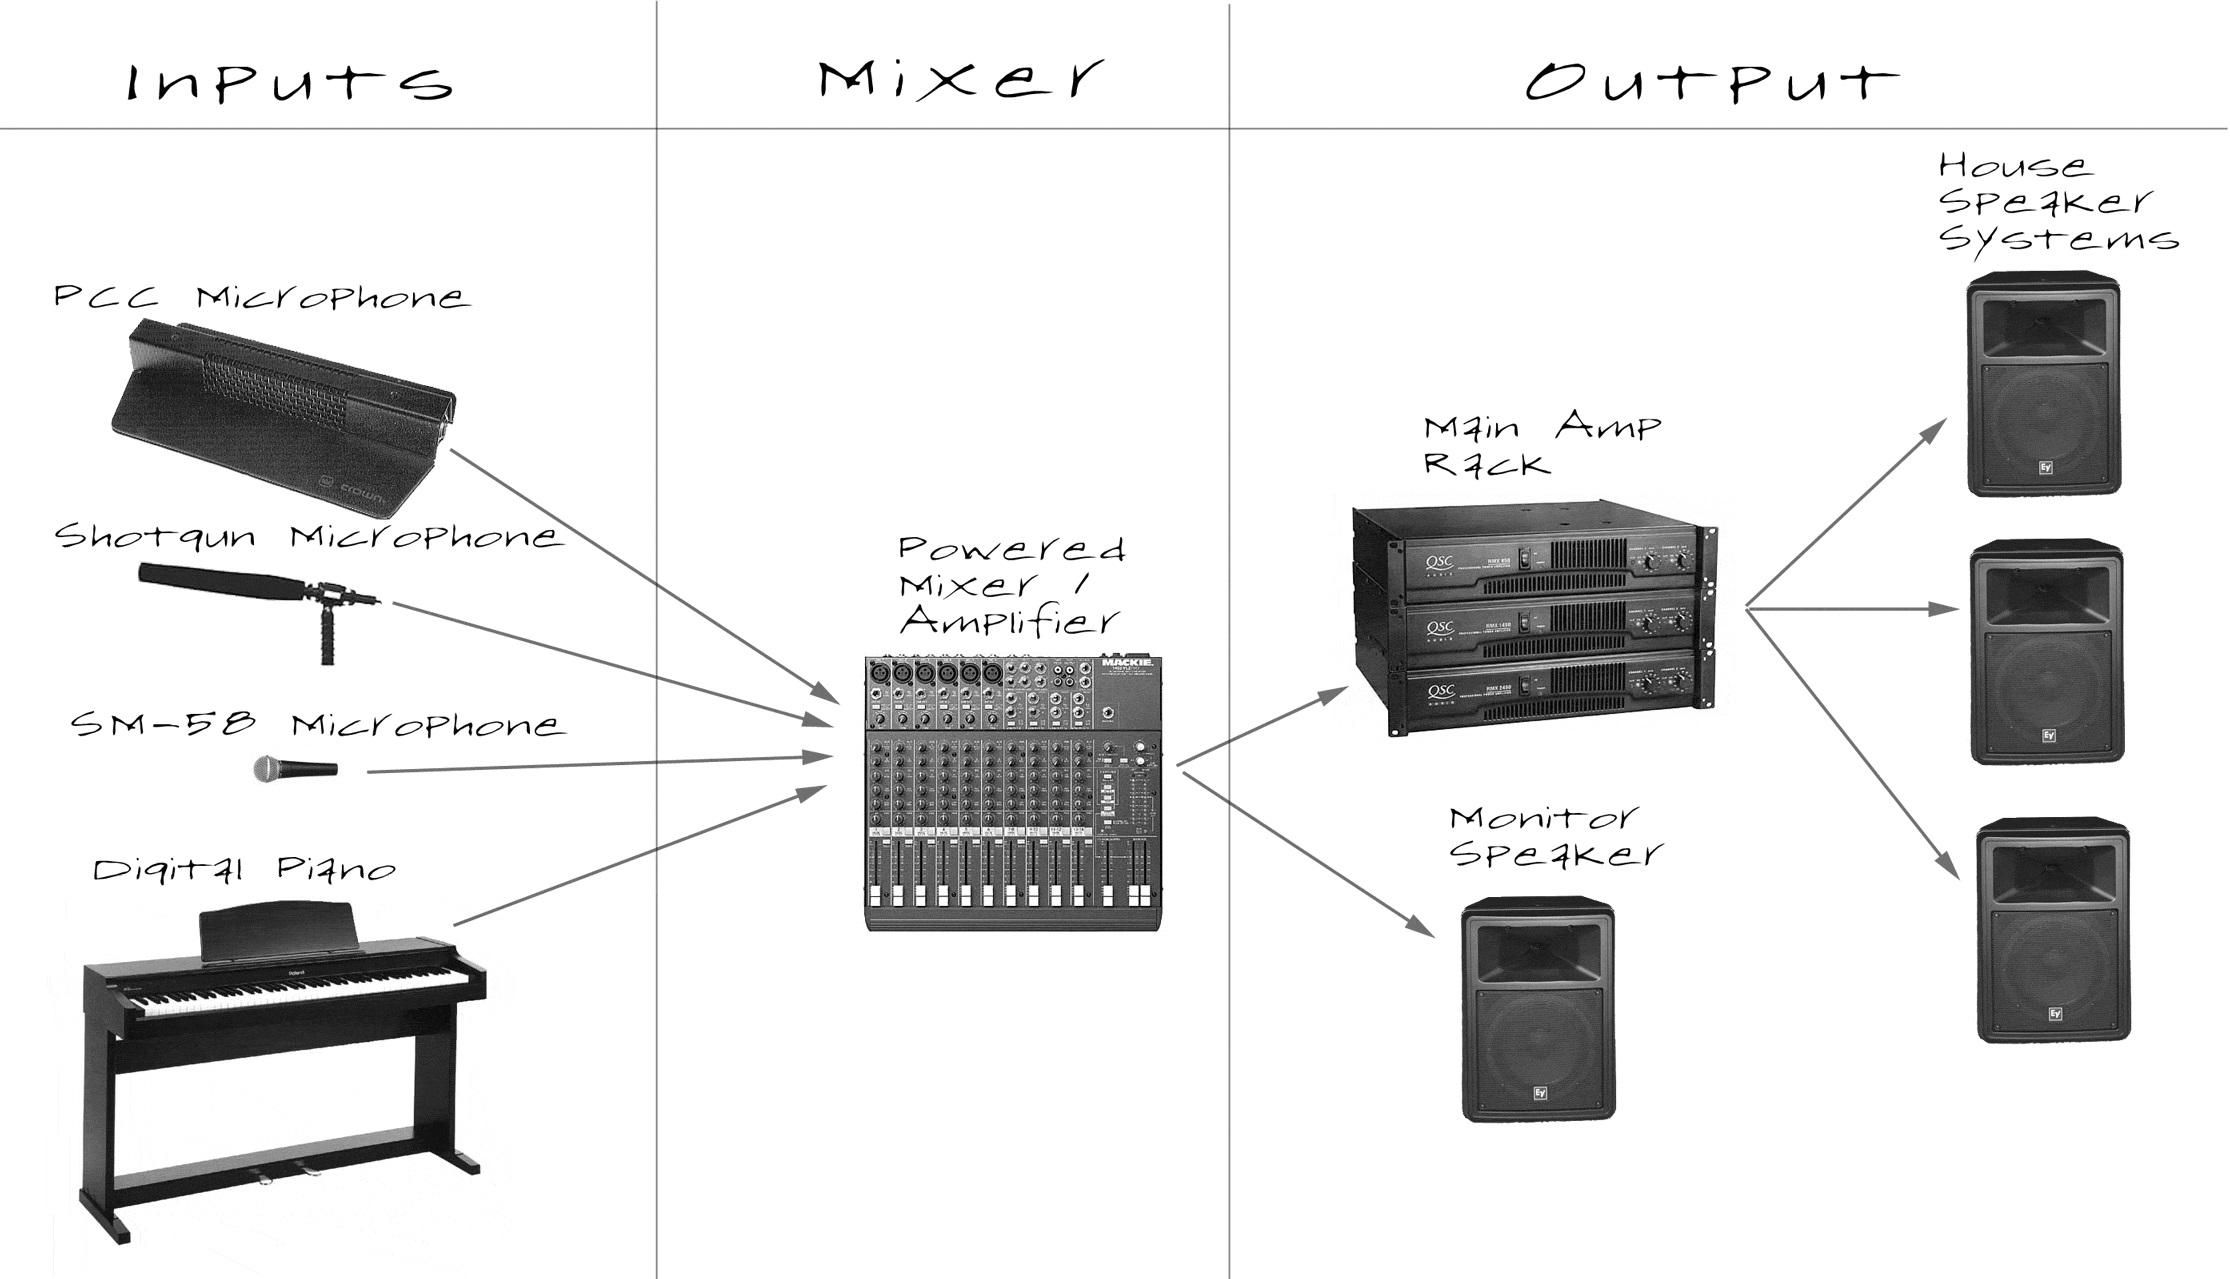
\includegraphics[width=18cm]{audio_labeled_diagram.jpg}
\caption{Basic structure of a sound system.}
\label{fig:intro}

\end{center}
\end{figure*}

The \textbf{INPUTS} section contains the different sources – basically anything that can make noise. We have to deal with a variety of sources, e.g. CD players, laptops, iPods, Microphones, DI boxes, etc. These all behave in slightly different ways which you will come across over time.

Then there is the \textbf{MIXER} section - it is possible to pass sound without a mixer, but then we have little or no control over it. Because we want to be able to combine signals together, the mixer is essential to creating an evenly balanced sound. They can also provide us with ways to route the signal to different sets of outputs (for example when mixing monitors for bands). Mixers, also called Mixing Desks, will be covered in more detail further on.

The first element in the \textbf{OUTPUT} section is the \textbf{power amplifier}. It increases the amplitude of the audio signal coming out of the mixer. Power amplifiers come in different shapes, sizes and power ratings. Last in the chain, after the amplifier, we have the \textbf{speakres} which turn the electrical signals from the amplifier into
sound waves. Speakers come in many flavours – some cover specific frequencies (e.g. subwoofers, or subs, which are designed to provide low frequency noise), some are designed to cover wide angles, while others are very directional. Speaker design is a bit of a dark art and there are some fascinating things that can be done!

It is worth noting that sometimes these elements can be combined together – sometimes you get mixers with built-in amplifiers (these are called powered mixers, we do not have any of these, but you may come across them), or more commonly, speakers sometimes have the amplifiers built in (these are called active speakers. If the amplifier is separate, it is a passive speaker.) The small Monacor PAs that we give to societies have a mixer, amplifier and speaker all built into one box. They are very neat, but generally less useful for our purposes!

\subsection{Signal Types}
\label{signal-types}
The electrical signals that travel through sound equipment come in a variety of sizes.
There are four main signal levels that you will need to know and understand. These are:

\begin{itemize}

\item \textbf{Microphone Level} - This is the level at which signal is sent out of a microphone. Because this is only voltage created by the movement of a coil within a microphone, it is very weak and therefore needs to be amplified using a pre-amp.

\item \textbf{Line Level} - This is the level at which professional audio equipment (CD players, mixing desks, DJ mixers, etc) outputs signal. It is much more powerful than microphone level and can be fed straight into an amplifier.

\item \textbf{Phono Level} - This is the level at which signal is generated by vinyl record decks as the needle bounces along the grooves of the record – it is a bit louder than microphone level, but still a long way from line level. Such signals have a
slightly stronger bass due to the mechanics of how they are generated. To compensate for this, they require special phono preamps which are built into most DJ mixers and some domestic hifi systems. It is not possible to connect them to other inputs, and if you connect a line level source to a phono preamp, it will sound distorted.

\item \textbf{Speaker Level} - This is the level at which amplifiers send out signal to speakers. It has to be powerful enough to make the speaker cone move and so is much more powerful than either microphone, line or phono levels. Speaker level signals should be treated with the same respect you would give mains power!

\end{itemize}


\subsection{Balanced and Unbalanced Signals}
\label{balanced-unbalanced}
As sound signals tend to be very small electrically-speaking, they are susceptible to interference from external sources (e.g. radio waves, electromagnetic sources like power cabling, lighting transformers etc). This usually manifests as a buzz, or as other noises, especially over a long cable. Balancing offers an efficient solution to this. Knowing the exact theory is not necessary, but it is very interesting. 

If you take a signal cable, and you introduce a source of interference, you end up with the same interference acting roughly equally on all the cores of the cable. This interference is then amplified by the preamps and amps in a system until it’s audible, as shown on Figure \ref{fig:dirty-signal}.

\begin{figure*}[h]
\begin{center}

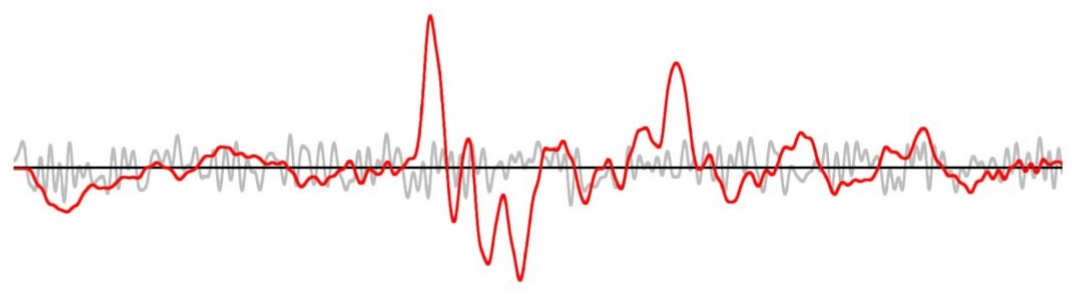
\includegraphics[width=18cm]{dirty-signal.png}
\caption{An image of a signal (shown in red) with some interference (shown in grey).}
\label{fig:dirty-signal}

\end{center}
\end{figure*}

Balancing involves sending an inverted signal along an adjacent cable core. This means that the same interference affects both signals, as shown on Figure \ref{fig:inverted-signal}.

\begin{figure*}[h]
\begin{center}

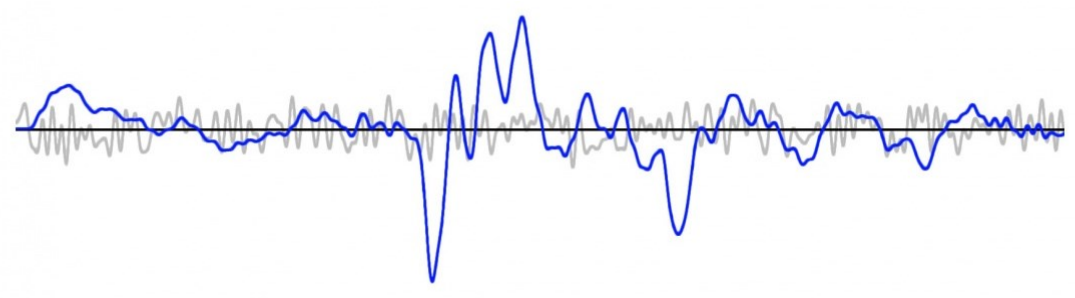
\includegraphics[width=18cm]{inverted-signal.png}
\caption{An image of the inverted signal (shown in blue) with the same interference (shown in grey).}
\label{fig:inverted-signal}

\end{center}
\end{figure*}

At the other end of the cable, the blue signal core gets inverted again, which flips both the signal and the interference, as shown on Figure \ref{fig:second-inverted}.

\begin{figure*}[h]
\begin{center}

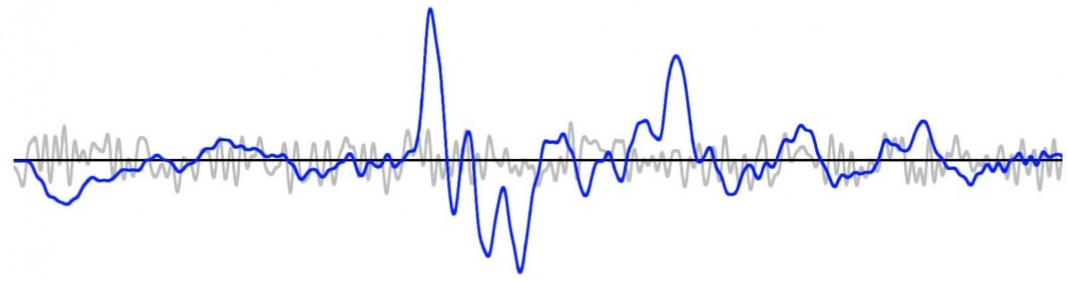
\includegraphics[width=18cm]{second-inverted.png}
\caption{An image of the re-inverted signal (shown in blue) with the now inverted interference (shown in grey).}
\label{fig:second-inverted}

\end{center}
\end{figure*}

If both the red and blue signals are added together, an even stronger version of the original signal is produced and the interference is canceled out, as shown on Figure \ref{fig:clean-signal}. This is a balanced signal. 

\begin{figure*}[h]
\begin{center}

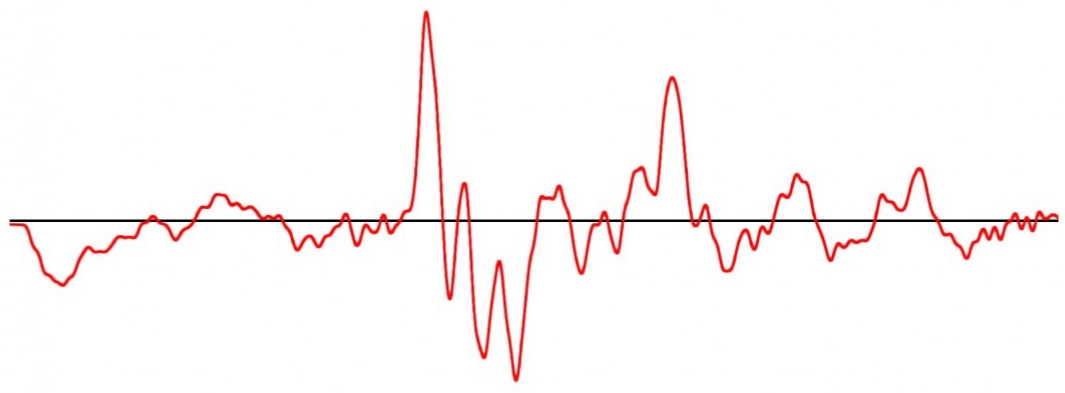
\includegraphics[width=18cm]{clean-signal.png}
\caption{An image of the produced stronger clean signal (shown in red) with no interference.}
\label{fig:clean-signal}

\end{center}
\end{figure*}

Thus a balanced signal is far less susceptible to noise and interference than an unbalanced signal.

\subsection{Balanced and Unbalanced Cables}
\label{balanced-unbalanced-cables}
As there are balanced and unbalanced signals, there are also balanced and unbalanced cables, i.e. cables that carry balanced and unbalanced signals, respectively.

A cable carrying \textbf{unbalanced signal} needs two cores - one of these is "ground" and the other carries the signal.

A cable carrying \textbf{balanced signal} needs three cores - ground, signal and an inverse copy of the signal. All the cores are wrapped around each other so that the external noise can affect them equally. 


\subsubsection{Balanced Cables}
\label{balanced-cables} 
There are two types of balanced cables that you will encounter in the Edinburgh University Students' Association:

\begin{itemize}

\item 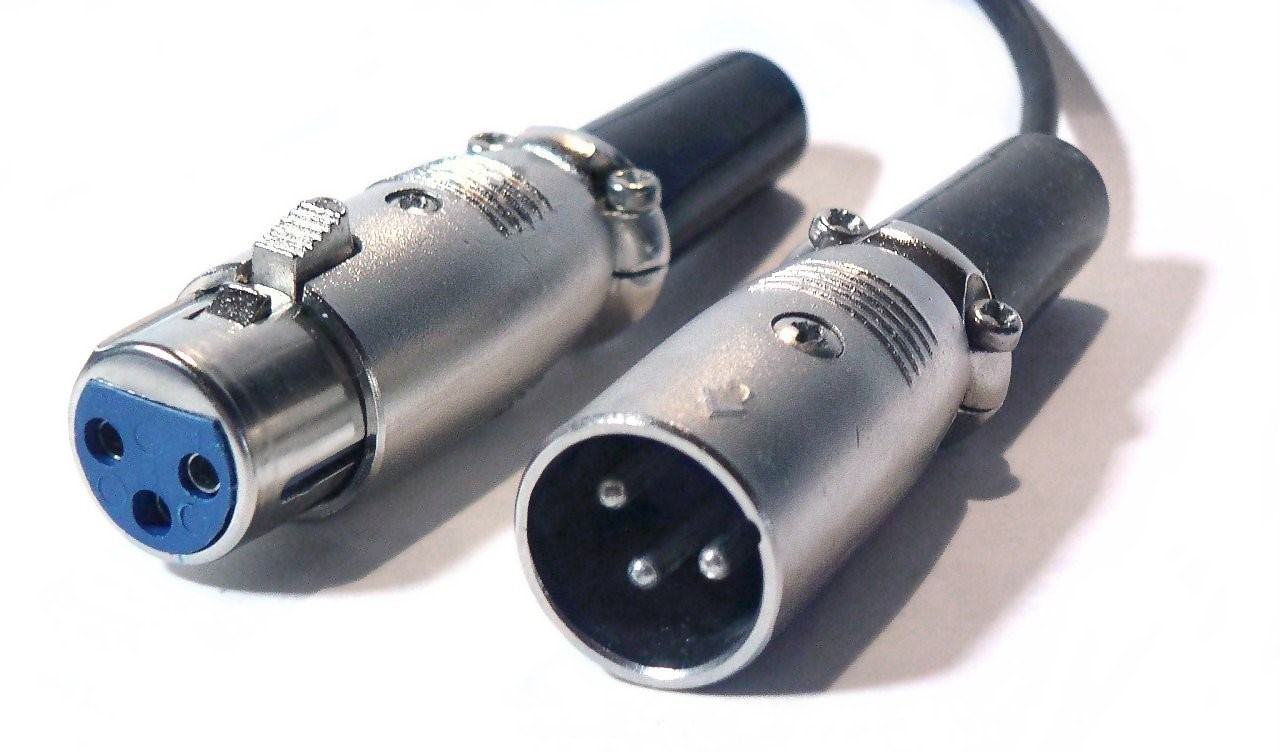
\includegraphics[scale=0.12]{xlr2.jpg}\textbf{XLR:} This is the most common type of cable in the sound world. Frequently referred to by musicians as "mic cable". Has three pins/holes.

\item 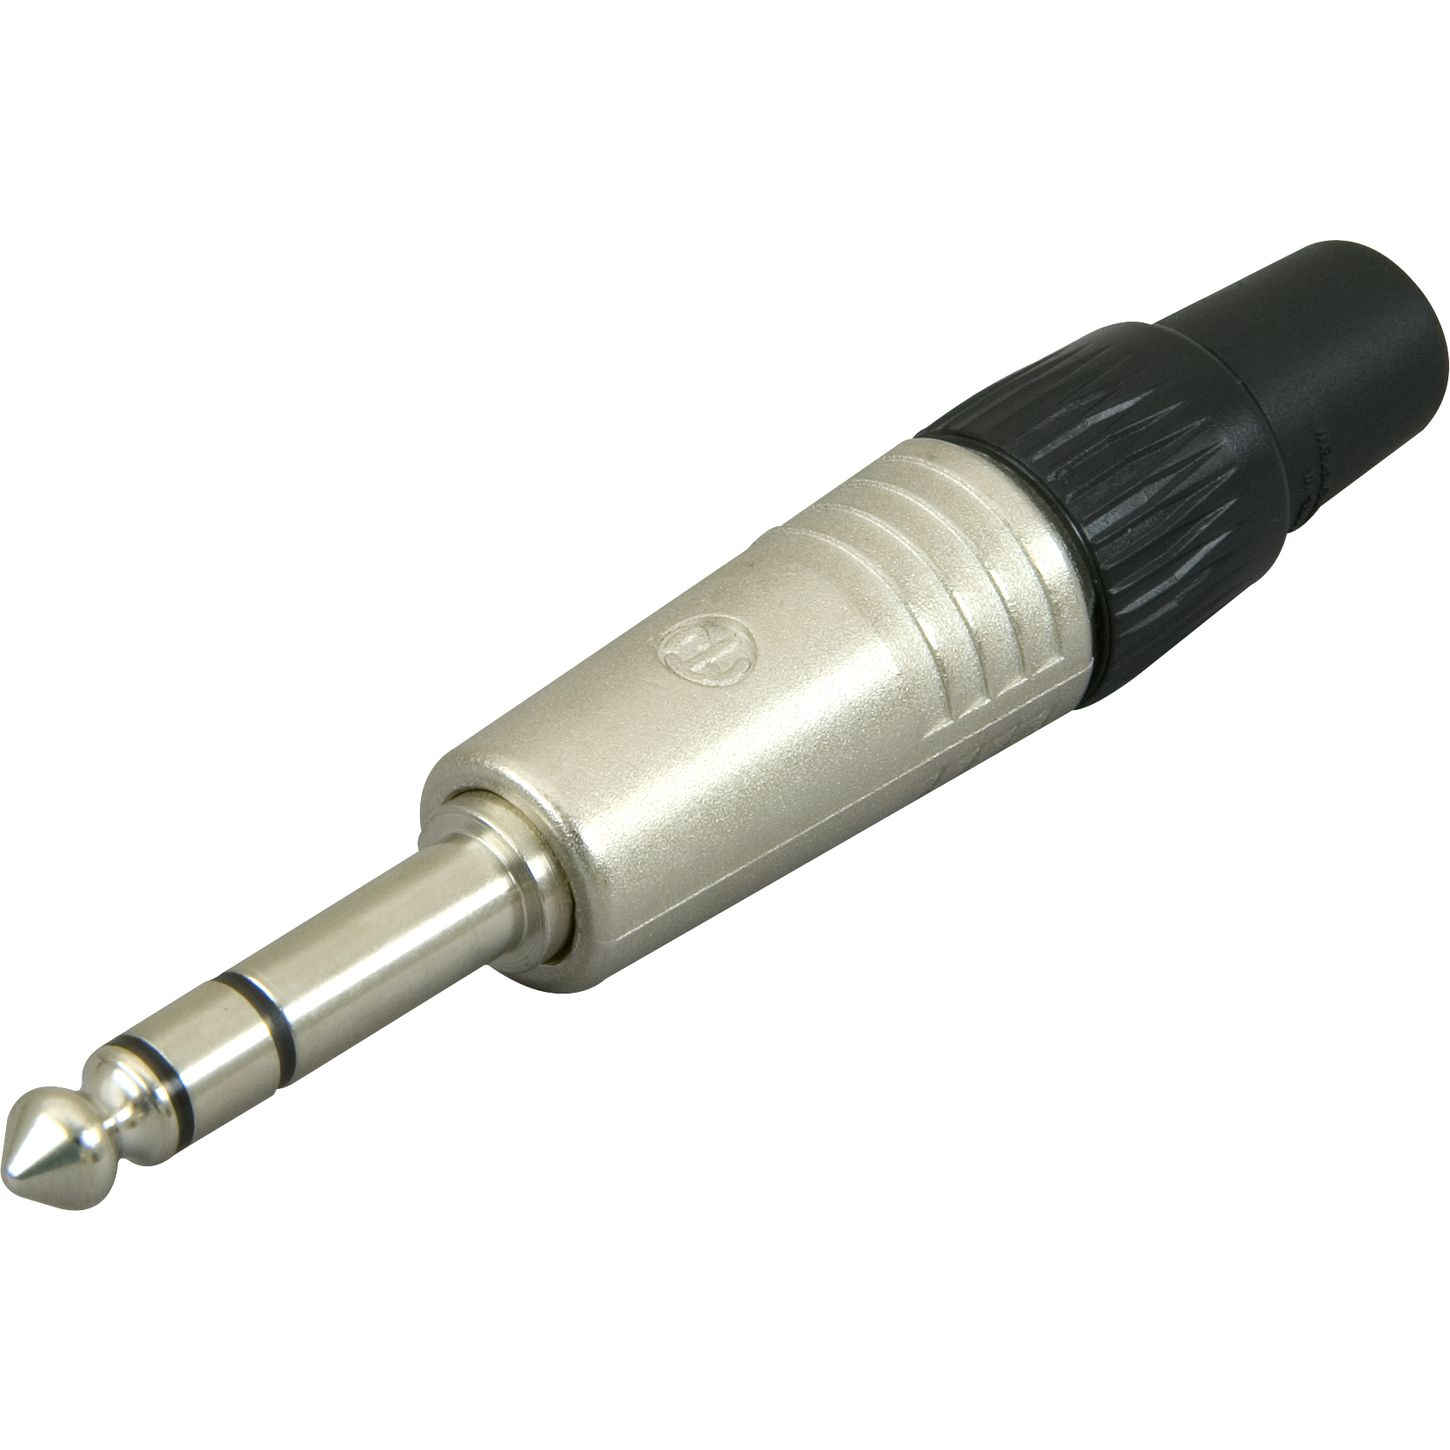
\includegraphics[scale=0.35]{bal_jack.jpg}\textbf{Balanced Jack (TRS):} This has three connections: tip, ring and sleeve. It is explained in more detail in the \textbf{Sound Training}. Not to be confused with unbalanced jack (guitar cable).

\end{itemize}


\subsubsection{Unbalanced Cables}
\label{unbalanced-cables} 
There are three types of unbalanced cables that you will encounter in the Edinburgh University Students' Association:


\begin{itemize}

\item 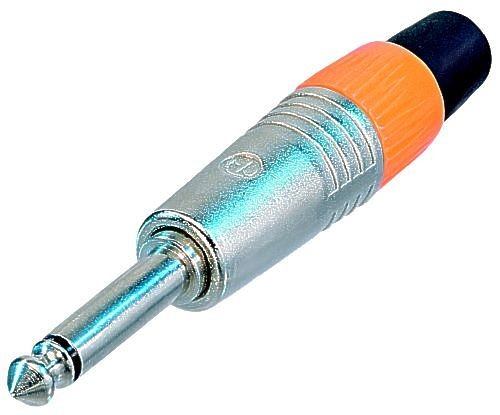
\includegraphics[scale=0.22]{jack_ts.jpg}\textbf{Unbalanced Jack (TS):} This has two connections: tip and sleeve. This is a guitar cable, do not confuse it with balanced jacks! Commonly known as 6.35mm or 1/4inch jack.

\item 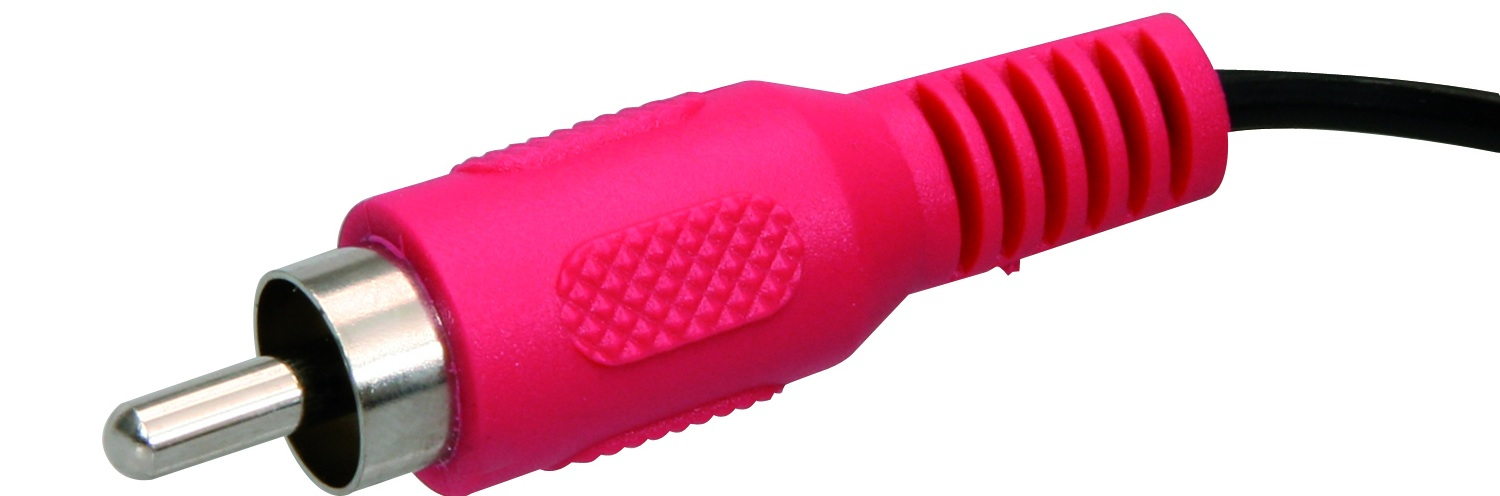
\includegraphics[scale=0.11]{rca.jpg}\textbf{RCA:} This is commonly used by DJ equipment, CD players, hi-fi types. Frequently referred to as "phono cable".

\item 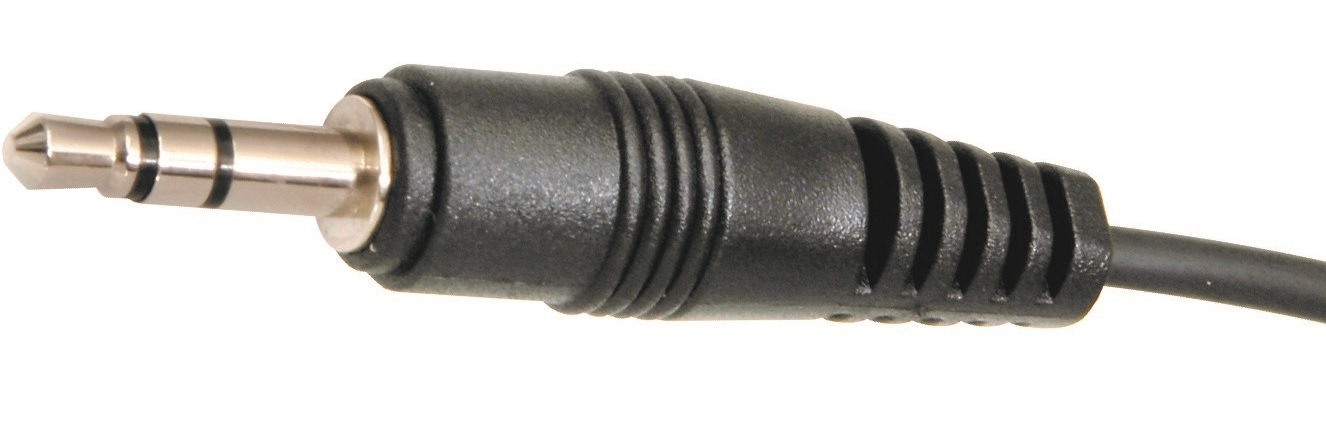
\includegraphics[scale=0.2]{minijack2.jpg}\textbf{Minijack:} This is used by laptops, iPods and other consumer equipment. Commonly referred to as an "aux cable", "3.5mm jack" or "Hi, can I play my laptop through your speakers?". Enjoys popping out mid-gig. Note that, while there are three connectors, it is unbalanced. This is because it carries stereo (two channel) signal. 

\end{itemize}

\subsubsection{Speaker Cables}
\label{speaker-cables} 
The previously presented cables carry microphone, line and phono level signals. However, cables are also needed to carry speaker level signals:

\begin{itemize}

\item 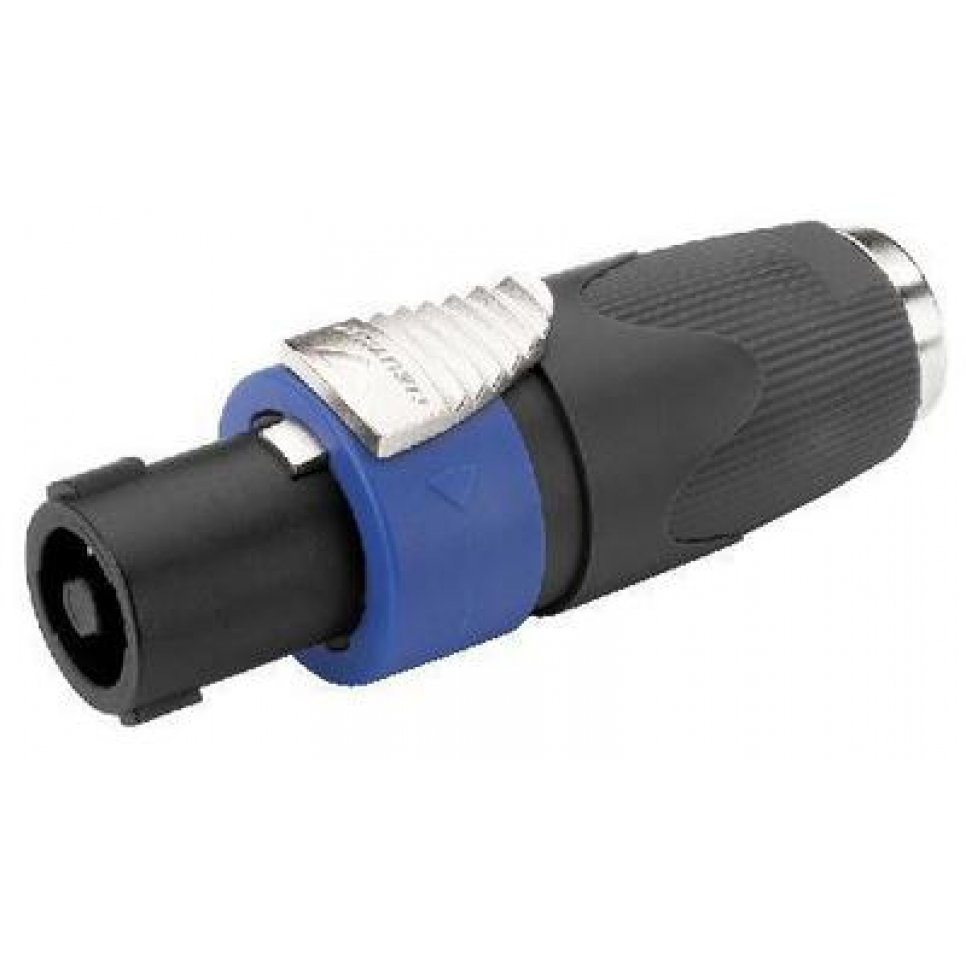
\includegraphics[scale=0.16]{nl2.jpg}\textbf{Speakon (NL2, NL4, NL8):} This is used to carry speaker level signal. Comes in several forms, with the number indicating the number of cores. The cores come in pairs, so NL2 can carry one signal, NL4 can carry two and NL8 can carry four signals.

\end{itemize}

\subsection{Mixing Desks}
\label{mixing-desks}
In audio, a \textbf{mixing console (mixing desk)} is an electronic device for combining (also called "mixing"), routing, and changing the volume level, timbre (tone color) and/or dynamics of many different audio signals, as produced by the devices presented in the \textbf{INPUTS} section of Figure \ref{fig:intro}. Figure \ref{fig:mixing-desk} provides a simple image of the workings of a mixing desk. Mixing desks can be either analogue or digital, depending on whether they work on analogue or digital audio signals. 

\begin{figure}[h]
\begin{center}

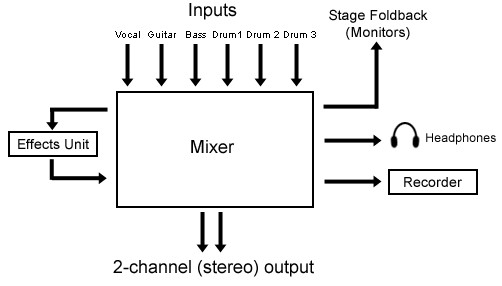
\includegraphics[width=9cm]{mixing-desk3.jpg}
\caption{A simple diagram of a standard mixing desk.}
\label{fig:mixing-desk}

\end{center}
\end{figure}

At the \textbf{Edinburgh University Students' Association} we have several mixing desks of different shapes and sizes. They are covered in more detail in the \textbf{Sound Training}. Here we use the \textbf{Midas Verona}, a.k.a. Matilda, as an example, as it is our most complex analogue desk. All analogue desks are based around the same concepts , although many remove or simplify a lot of the features. We shall now look at the two types of sections an analogue mixing desk has - \textbf{Channel Strip} and \textbf{Master Section}.


\subsubsection{Channel Strip}
\label{channel-strip}
A channel on a mixing desk is responsible for a single input, which could be a microphone, DI box, etc. Consequently, on analogue desks, the number of channels limits the number of inputs you can have. The cahnnel strip gives you control to change the amplitude of the input signal, change its sonic attributes and deside how it will be mixed along with the other channels. A detailed description of the channel strip is provided on Figure \ref{fig:channel-strip}.

\begin{figure}[H]
\begin{center}

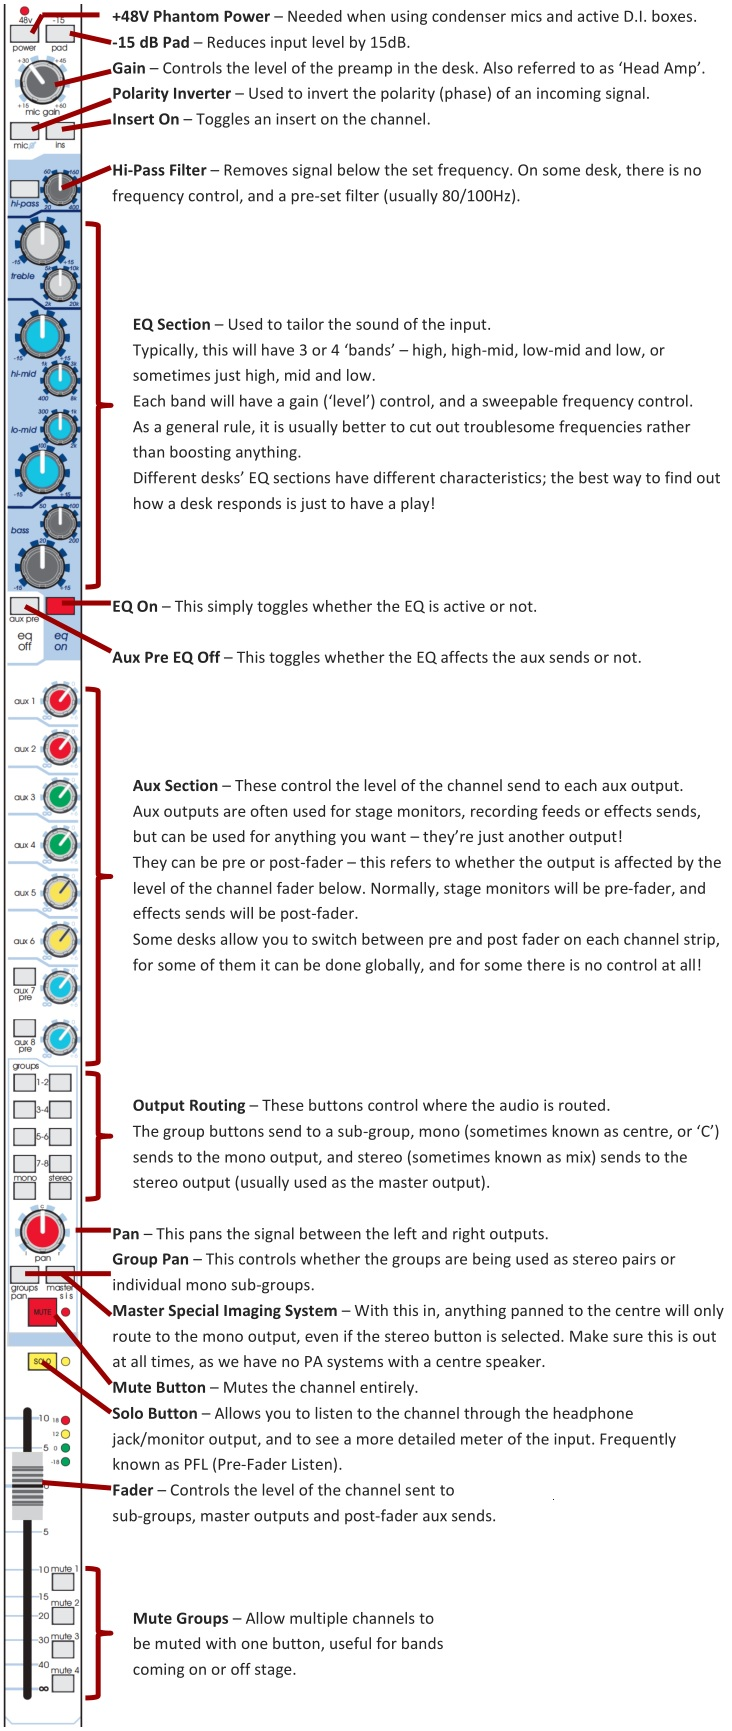
\includegraphics[width=10cm]{channel-strip.jpg}
\caption{An image of a standard mixing desk input strip.}
\label{fig:channel-strip}

\end{center}
\end{figure}

\subsubsection{Master Section}
\label{master-section}
The master section is where all the master volume controls for each output can be found. On the Midas Verona, it is separated into two parts - \textbf{Auxiliary (AUX) Master Section}, shown on Figure \ref{fig:aux-section}, and \textbf{Main Master Section}, shown on Figure \ref{fig:master-section}.

\begin{figure}[H]
\begin{center}

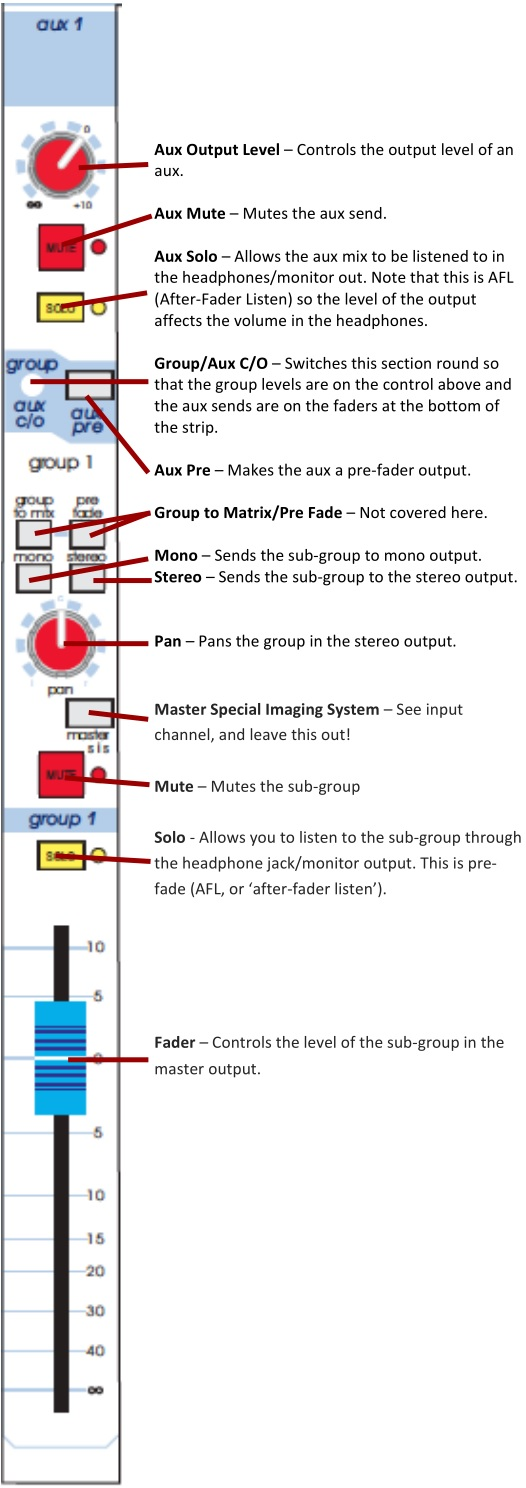
\includegraphics[width=8cm]{aux-section.jpg}
\caption{An image of the Auxiliary (AUX) Master Section.}
\label{fig:aux-section}

\end{center}
\end{figure}

\begin{figure}[H]
\begin{center}

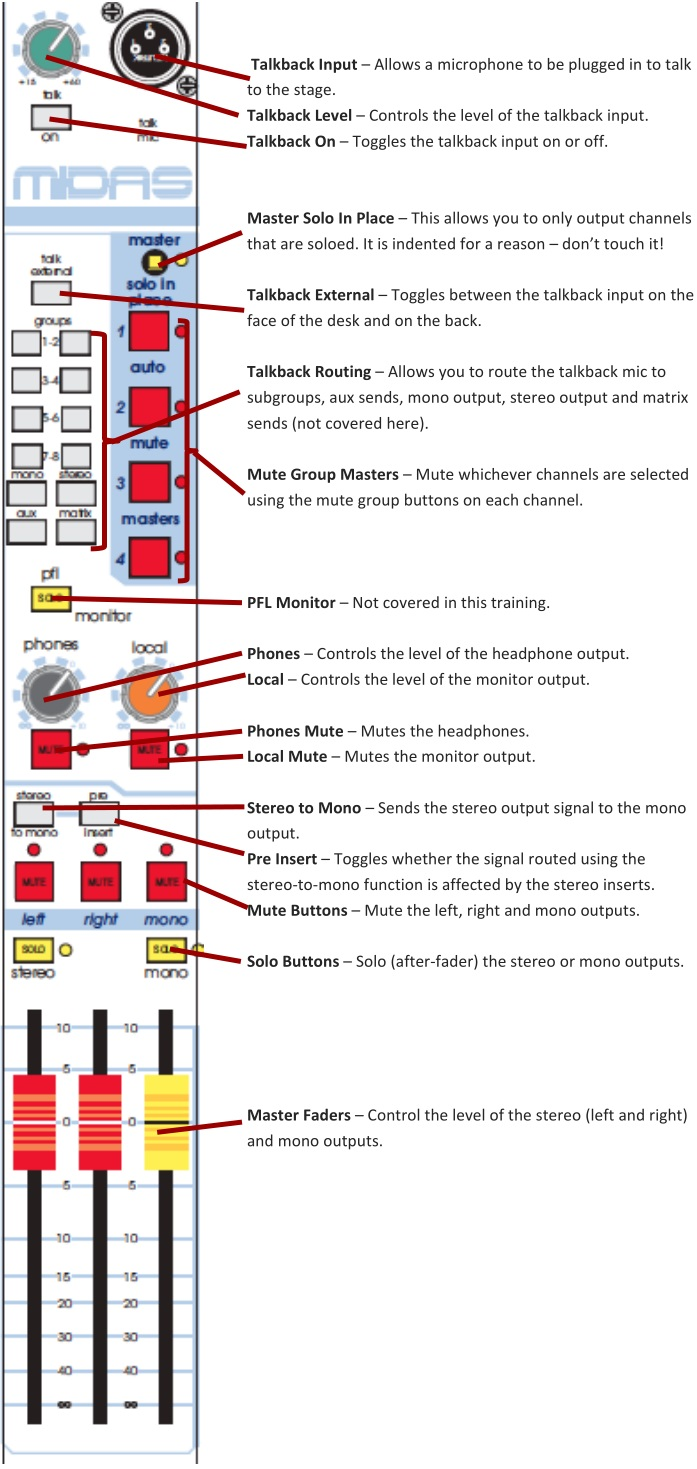
\includegraphics[width=10cm]{master-section.jpg}
\caption{An image of the Main Master Section.}
\label{fig:master-section}

\end{center}
\end{figure}


\section{Lighting}
\label{lighting}
Stage and club lighting is a strange and complex world of smoke and mirrors – and moving heads, PAR Cans, DMX and dimmers. The basic lighting course is intended to introduce you to lighting, and give you a grounding in the basic concepts and equipment used. By the end of the day you should be able to identify various different sorts of light, and understand how they are controlled.

This document is intended as a companion to the session, to allow you to revise on your own if you want to. It is by no means comprehensive, and is no substitute for the genuine knowledge and experience you can only gain over time.

\subsection{Types of fixtures}
There are two main categories into which stage lighting falls. Generic lighting, and intelligent lighting. The main difference is the method of supplying power to and controlling the fixture (or lantern, luminaire, light, etc.)
Within these categories there are a number of sub categories.

\subsubsection{Generic fixtures}
Generic lights are similar to the everyday lights you have in your home. They consist of a lamp, like a specialised sort of lightbulb, in some sort of metal casing. Different sorts of generic lights have lenses and other features to alter the light that comes out of them. They don’t have any sort of built in control, and although some are very versatile, they must be adjusted manually every time you want them to do something different.

Generic lights are controlled by plugging their power into a dimmer; this allows the brightness of the light coming out to be controlled. A lighting desk is used to tell the dimmer what to do. Generic lights almost always produce white light in a round (or roundish) shape, which is then coloured using gel, a sort of clear plastic material which is placed in front of the beam of light. The shape of the beam can also be altered by obstructing parts of the beam, either with metal shutters or with specially shaped gobos, which can be used to project images.

Intelligent lights differ from generic lights in that rather than plugging them into a dimmer, they are plugged straight into the mains. The control cable from the lighting desk plugs directly into the light and tells it what to do. 
\textbf{Intelligent lights do not need to be plugged into dimmers, and indeed they are likely to be broken if you try!}

\begin{itemize}
\item \textbf{PAR Can} (or Parabolic Aluminized Reflector luminaire) 

\begin{figure*}[h]
\begin{center}

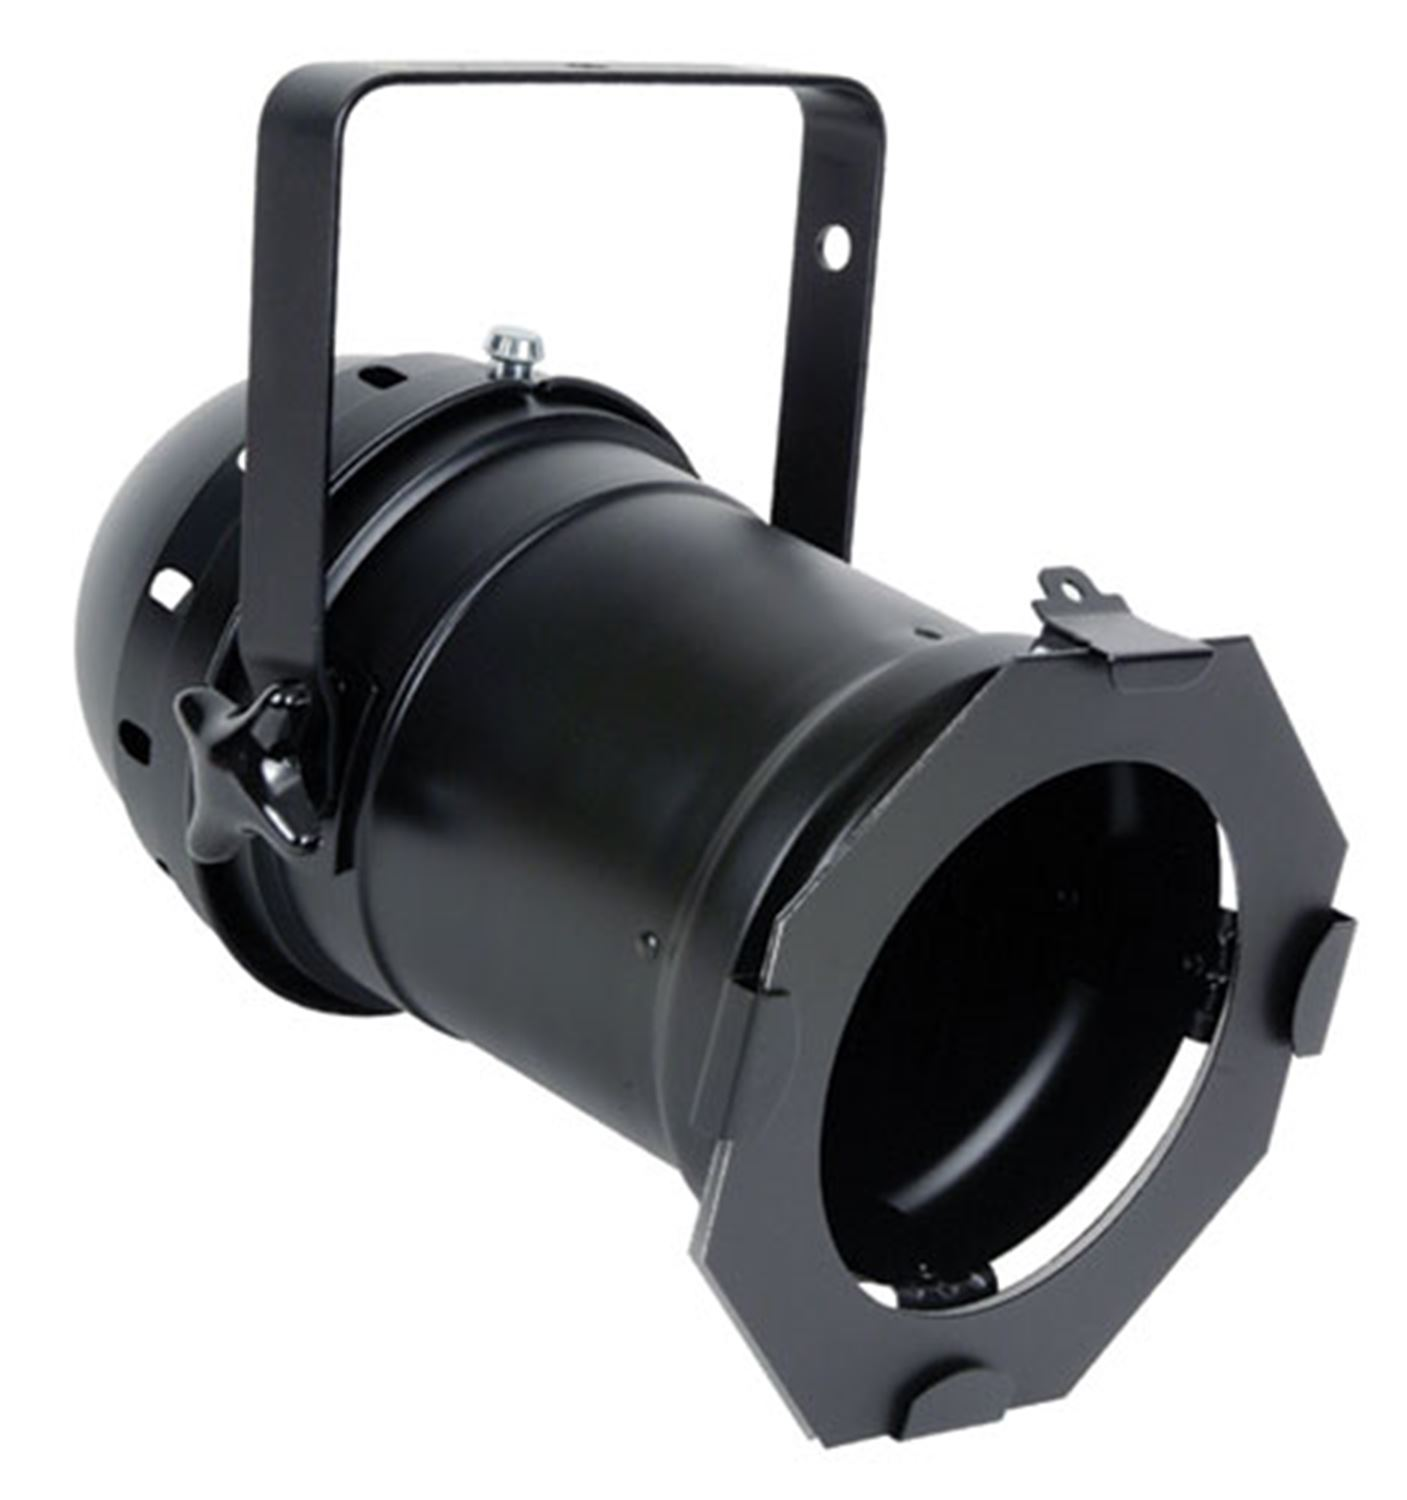
\includegraphics[height=5cm]{PAR64.jpg}
\caption{PAR 64 Can}
\label{fig:par64}

\end{center}
\end{figure*}

A PAR Can is basically a bucket with a lamp in it. 
It’s one of the most basic sorts of light; it produces a high intensity and unfocussed beam of light that can be coloured using lighting gel. 

The lens and reflector are built into the lamp, and as such are fairly basic, as they are thrown away - or recycled - every time a lamp blows.
A number of different lamp types are available, with different power ratings and optical properties. The most common lamps that you’ll encounter at EUSA are the CP60 (A very narrow spot), the CP61 (A narrow spot) and the CP62 (Medium flood).

The lamps are held into the fixture with a sprung metal clip, and lamps with an oval beam can be rotated to adjust the beam. The lamps are plugged into the cable using a ceramic connector.

There are also different sizes of PAR Can shell, ranging from the tiny PAR16 “birdie” (under par!), through PAR38 and PAR56 to the large PAR64. The number is the diameter of the lamp in eighths of an inch (PAR64 is therefore 8” diameter)

PAR Cans are very popular for lighting bands, as they produce a simple and striking look, but appear pretty much everywhere within lighting. They come in many sizes, which vary in power requirements and brightness. The most common is the PAR64, a bright 1kW fixture. There are many of these in the Debating Hall, Pleasance Theatre, Potterrow Venue, and some elsewhere.

\textbf{Common faults:}
\begin{itemize}
\item The construction of the fixture is cheap, and so connections can easily become dodgy. It is worth confirming that the ceramic has not become loose. Give it a wiggle.
\end{itemize}

\item \textbf{Fresnel:} 

\begin{figure*}[h]
\begin{center}

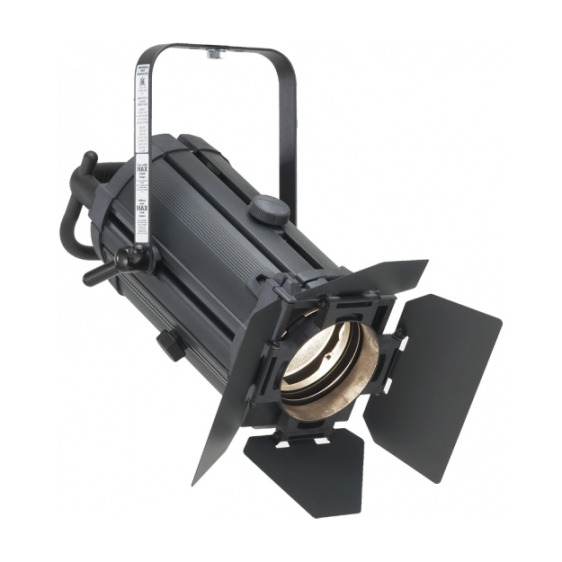
\includegraphics[height=5cm]{acclaim.jpg}
\caption{An Acclaim Fresnel}
\label{fig:fresnel}

\end{center}
\end{figure*}

A Fresnel (freh-nel) produces a soft-edged beam of light, which is generally quite wide, using a single lens. 

They are used to light large areas evenly, for example when creating a “stage wash” to make an entire stage visible. 

They can be crudely focused using external shutters called “barn doors” which block part of the beam, and they can be coloured with gel. 
The beam can be made larger or smaller by moving the lamp backwards and forwards relative to the lens within the casing. 
Many manufacturers make different sort of fresnels, and they vary widely depending on make and model.

\begin{figure*}[h]
\begin{center}

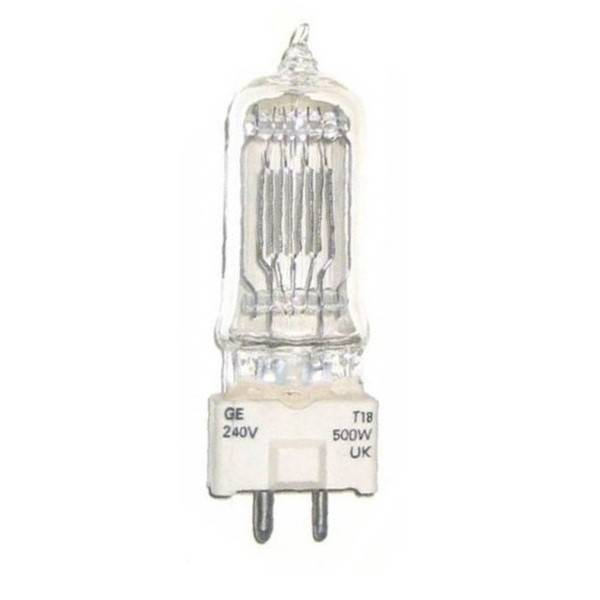
\includegraphics[height=5cm]{t25.jpg}
\caption{A T25 lamp, used in fresnel fixtures}
\label{fig:fresnel-lamp}

\end{center}
\end{figure*}

We have 500W (T25, pictured in Figure \ref{fig:fresnel-lamp}), 750W (HPL) and 1kW (T19) models, which can also take 650W (T26/T27) and 1200W (T29) lamps.

\textbf{Common faults:}
\begin{itemize}
\item Warm the lamp up before changing the focus. If you can’t change the focus easily, turn the fixture off and check it moves freely before turning it on again.
\item Don’t touch the lamp with your fingers. Use the instruction leaflet if you need to touch the glass.
\end{itemize}

\item \textbf{Profile: }
A profile uses a pair of lenses to enable it to produce a sharply defined beam with a hard edge. Some, such as the Source Four fixtures owned by EUSA, have special internal shutter blades to allow the beam to be shaped accurately. Some have a fixed beam size, eg. 50\textdegree, 36\textdegree, 25\textdegree, etc., whereas others have a zoom function which allows the beam size to be varied. 

\begin{figure*}[h]
\begin{center}

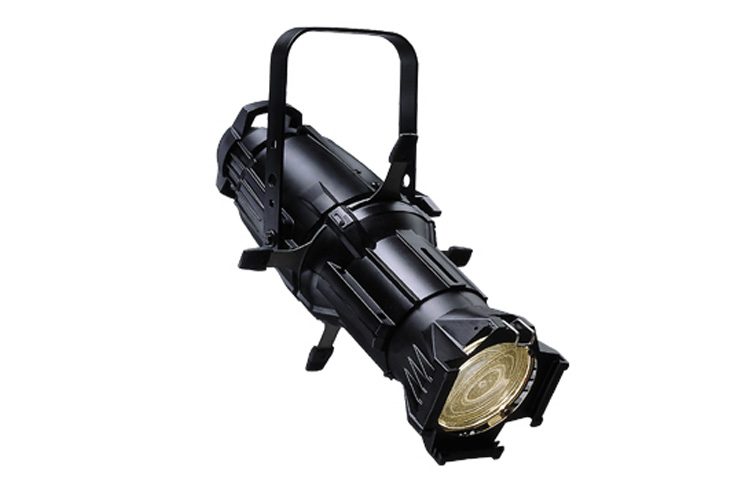
\includegraphics[height=5cm]{source4.jpg}
\caption{Source 4 Profile}
\label{fig:profile}

\end{center}
\end{figure*}

Figure \ref{fig:profile} is an ETC Source Four Profile, a very popular lantern, which we have primarily in the Debating Hall and Pleasance Theatre.

They can also be used to project images or patterns using a gobo, which is either a metal disk with holes in it to let the light through or a glass disk with a pattern printed on it. They can also be coloured using gel. They are among the most flexible of generic lights, with many applications. 

\textbf{Common problems:}
\begin{itemize}
\item Don't touch the lamp. Use the leaflet.
\end{itemize}

\end{itemize}

\subsubsection{Dimmers}
A dimmer is required to allow the brightness of a generic light to be controlled. It takes mains power in and distributes it to circuits, altering the power to change the light output of the fixtures running from those circuits. It is also connected to a lighting desk by a cable that carries DMX control information (more about this later), which tells the dimmer how bright the lights should be. 

These are referred to as “channels” and each has a limit on how many lights can be plugged into it, depending on how much power the dimmer can supply relative to how much each light needs.

Generally it’s best to aim for one channel of dimming per lantern, as this gives the greatest measure of control over the lighting.

There are installed dimmers in the Underground, Debating Hall, Potterrow, and Pleasance Theatre.

\textbf{Common problems:}
\begin{itemize}
\item	Make sure it’s turned on (!)
\item	Check the fuses
\item	Check the DMX connection indicators
\item	Check the DMX address
\end{itemize}

\subsection{Intelligent fixtures}

\subsubsection{Moving heads}

Moving heads are the largest and most complicated of intelligent lights. The body of a moving head is held in a special yoke, which allows it to move to point in almost any direction, as well as creating striking moving effects.	They are popular for lighting live bands and nightclubs.

\begin{figure*}[h]
\begin{center}

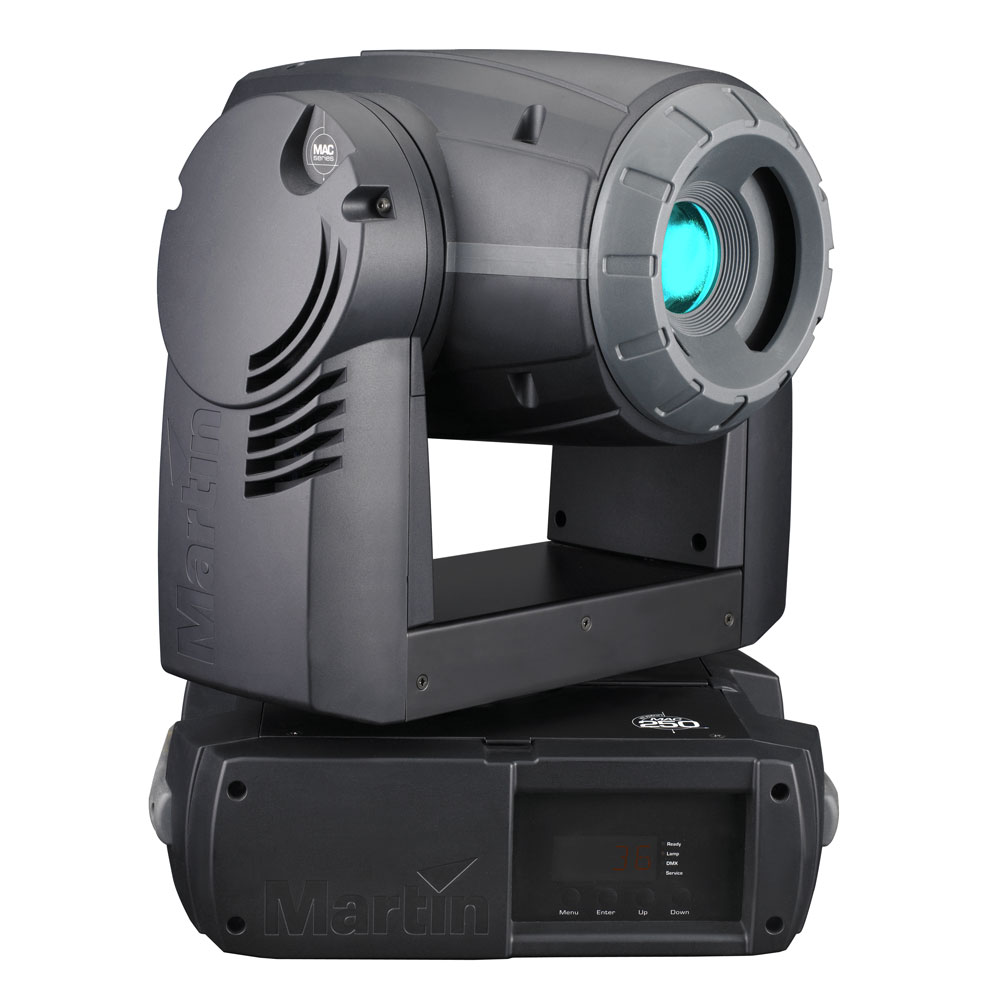
\includegraphics[height=5cm]{mac250krypton.jpg}
\caption{Martin MAC 250 Krypton}
\label{fig:krypton}

\end{center}
\end{figure*}


Moving heads, or “movers”, come in three basic varieties, washes, beams and spots. They also come in combinations of the three (wash-beams etc). Washes are broadly similar to a generic fresnel giving a wide soft beam, and spots are broadly similar to generic profiles giving a narrow sharp beam.

Rather than having gels and gobos which have to be manually changed, movers have colour and gobo wheels which hold several different colours and gobos internally and which can be controlled remotely from a lighting desk. Some moving heads also have a feature called colour mixing, which means they can reproduce almost any colour. Rather than using a dimmer pack, movers dim using a metal shutter which can also be used to rapidly strobe the light on and off. There are various other effects and features possessed by some moving heads such as beam-splitting prisms

\textbf{Common problems:}

\begin{itemize}
\item Check the DMX connection indicators
\item Check the DMX address
\end{itemize}

\subsubsection{Scanners}

Scanners are generally smaller and less complicated than moving heads, and are commonly found in nightclubs. Rather than moving the entire body of the light, they bounce the beam of light off of a movable mirror. This means that the light is slightly less bright and that the beam cannot move in as wide a range. On the plus side, they are far cheaper, weigh less than moving heads, and can move faster. They only come in profile versions and usually have gobo and colour wheels, and sometimes shutters. 

Figure \ref{fig:scanner} is Martin MX-1, a scanner which EUSA has 4 of, currently located in the Underground.

\begin{figure*}[h]
\begin{center}

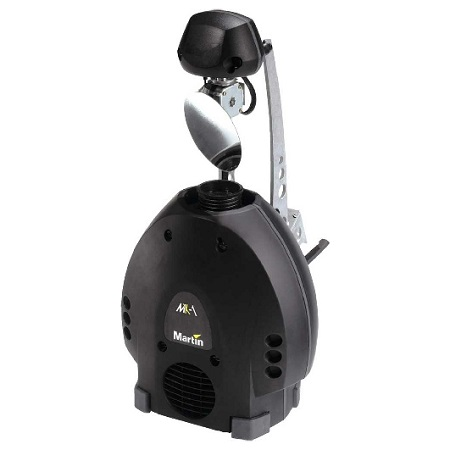
\includegraphics[height=5cm]{mx1.jpg}
\caption{Martin MX-1 Scanner}
\label{fig:scanner}

\end{center}
\end{figure*}

\textbf{Common problems:}
\begin{itemize}
\item 	The mirrors break very easily. Be careful when handling
\item	Check the DMX connection and address
\end{itemize}

\subsection{LED fixtures}

\begin{figure*}[h]
\begin{center}

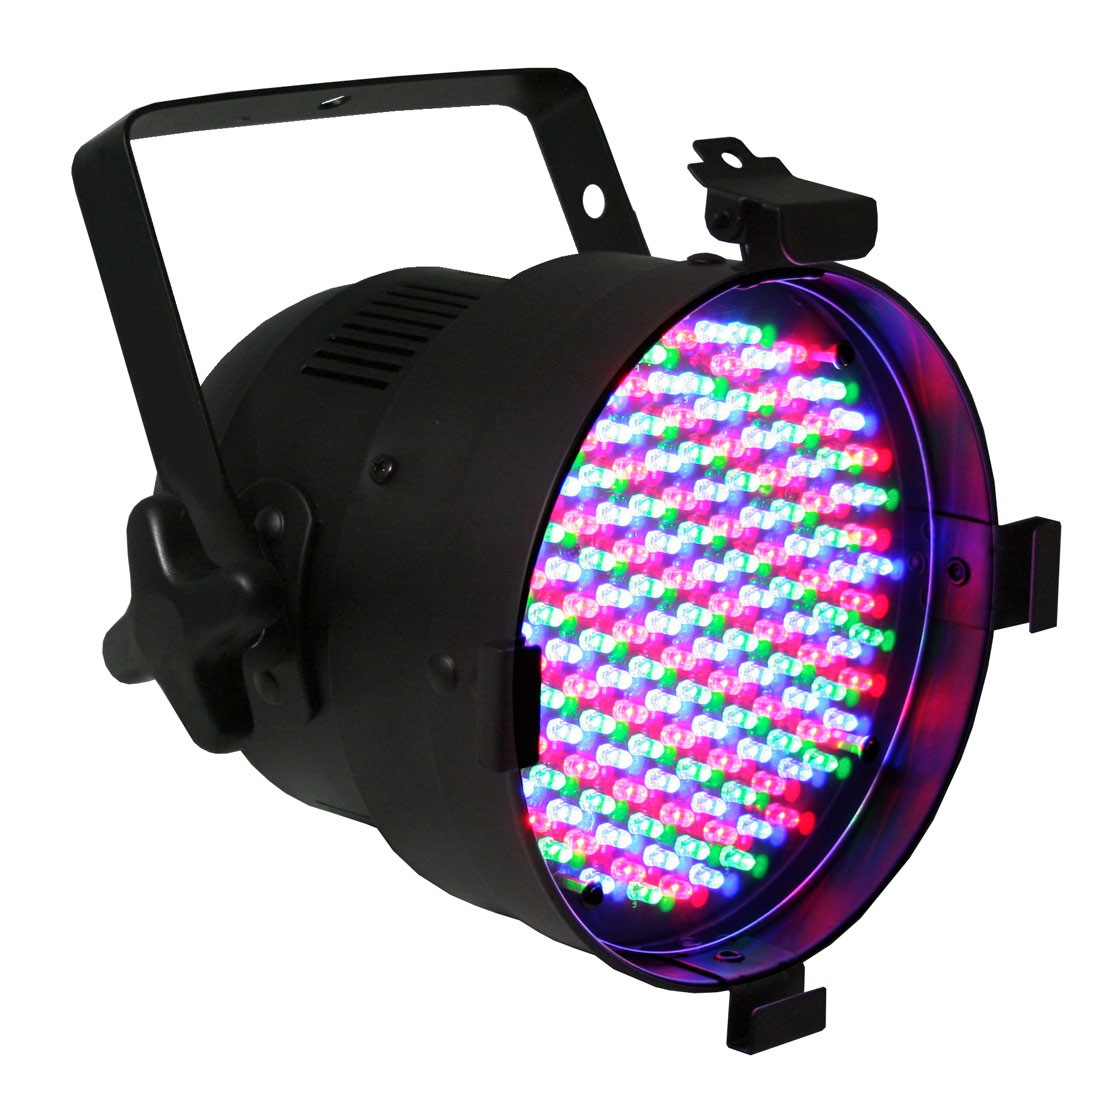
\includegraphics[height=5cm]{ledpar.jpg}
\caption{LED PAR 56}
\label{fig:ledpar}

\end{center}
\end{figure*}

While LED Fixtures are technically intelligent lights (i.e. require a control input), they have some common traits that are worth mentioning separately.

Most of our LED fixtures contain red, green and blue LEDs. By altering the intensity of each of these colours, it is possible to make virtually any colour of light. Most LED fixtures therefore have at least 3 DMX control channels for the three colours, and sometimes have additional channels for strobe effects or colour macros. 

\textbf{Common problems:}
\begin{itemize}
\item	Check the DMX connection and address
\end{itemize}

\subsection{Effects}

As you're probably aware, there are some very exciting effects that augment the generic and intelligent fixtures talked about above. These include things like smoke, haze, heavy fog, pyrotechnics, strobes and UV. Most of them are a bit hazardous if misused or overused, so it's important to use common sense when using them to make sure nobody could get hurt.

\begin{itemize}
\item \textbf{Smoke} (or fog) machines are probably the most common kind of effect. They produce a solid burst of thick, white smoke into the venue which then disperses out into a fog-like effect. These are great for nightclubs, as they introduce another dimension into the room and generally excite the crowd on the dancefloor. They also have potential uses in theatre and come in all shapes and sizes with different kinds of attachments. They operate by heating up a glycol solution and pumping it through a nozzle at high pressure. Be careful when filling them as the fluid can be an irritant for some people, and it's very slippery if spilled!

\item \textbf{Low foggers} work on the same principle as a normal smoke machine, but once the smoke has been created it is passed over an icebox or refrigerated coil cooling it down and making it hover just above the floor. These are great for spooky Halloween effects!

\item \textbf{Haze Machines} (or hazers) work on the same principle as smoke machines, but use a different formulation of fluid in combination with a fan to create a much finer 'mist' effect. This haze is quite unobtrusive, but is great for picking out the beams of lights through thin air making lighting displays look more vibrant and three-dimensional. 

\item \textbf{Strobes} are lights that are designed to flash on and off rapidly. They can cause disorientation, and some people believe they can be a cause of epileptic seizures. For this reason we have to display warnings at the entrances to our venues, and we’re also obliged to keep the use of them to “reasonable” levels.

\item \textbf{UV} lights produce a deep purple ultraviolet light that reacts with special paints, and makes white surfaces show up. They’re particularly loved by groups of goths and ravers, but look quite cool for other things too!

\item \textbf{Pyrotechnics} come in all kinds of different designs and sizes. These are basically indoor fireworks/explosive effects that can wow the crowd! Some go “bang”, some go “fizzle”, and some fire confetti everywhere! As with all explosives, these are very dangerous and are strictly regulated by the council and local fire brigade. 

\item \textbf{Decor} is not to be underestimated either – A tasteful swag of fabric or a full set of beach related paraphernalia can make all the difference to an event, introducing a theme or just a splash of colour. Fabrics should be treated with a flame suppressant such as Flamebar, which can be sprayed on to the material.

\end{itemize}

\subsection{DMX}

DMX512 (Digital Multiplex) is the most common communication protocol used by lighting fixtures. This protocol is usually transmitted along XLR cable with 5- or 3-pin connectors on the end, and can be daisy-chained between fixtures. Each “universe” can carry up to 512 channels of information. The address of the fixture tells it which channel(s) of data to listen to. Every lighting attribute (dimmer, gobo wheel, colour etc.) will respond to its own control channel, offset from the fixture address. 

DMX signals are very robust, and will work through most fault scenarios, however there are some basic rules to follow when running the cabling: There’s a maximum number of fixtures that you can chain together before the signal begins to lose strength. This number is nominally 32, but can vary depending on some other factors. DMX needs to be split using “active” splitter devices which will buffer and boost the signal. The ends of lines should be terminated using special terminator plugs – in most cases you won’t run into any issues without a terminator, but it’s good practice to stick them in - especially if you see any unexpected behaviour from the fixtures!

There are three ways that the address of a fixture or effect can be set:

\begin{itemize}

\item \textbf{Using DIP switches}

DIP switches are banks of little switches. The switches work on a binary number system, ie: each switch represents double the value of the one next to it. These are generally used on older fixtures and are a wee bit fiddly to set – something pointy will probably be required!

\begin{figure*}[h]
\begin{center}

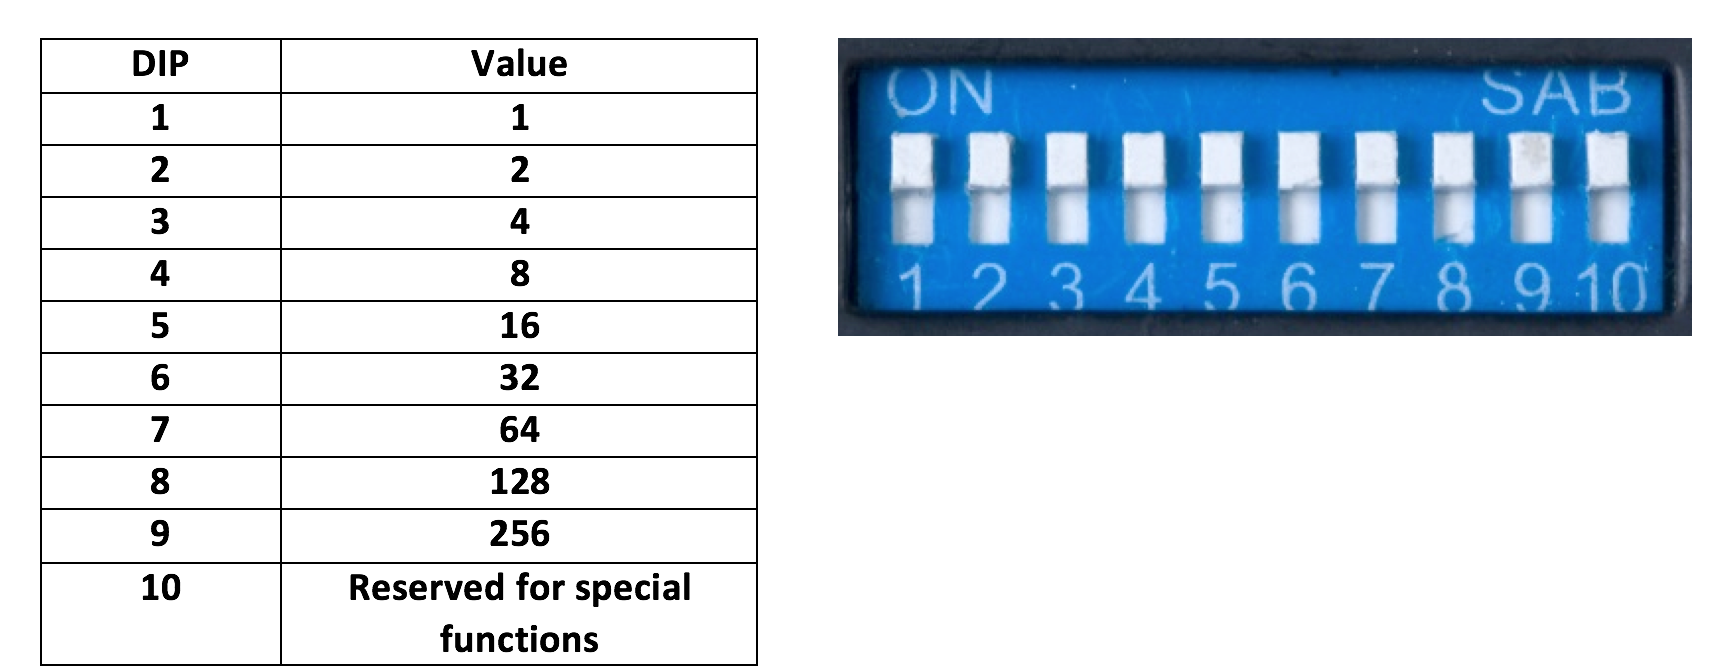
\includegraphics[height=5cm]{dip.png}
\caption{DIP switches and their values}
\label{fig:dip}

\end{center}
\end{figure*}

The values of each switch are in Figure \ref{fig:dip}.

Now to get from these values to a DMX address, it’s a simple case of addition. For example:
(DIP switch numbers are in brackets)
\begin{itemize}
\item	DMX $3 		= 	2  (2)   +   1  (1)$
\item	DMX$ 11			= 	8  (4)   +   2  (2)$
\item	DMX $135 	=	128 (8)  +  4 (3)  +  2  (2)  +  1  (1)$
\end{itemize}

Alternatively, you can using a DIP switch calculator. These are small apps that can be downloaded for your smartphone that will do the job for you.

Note that some cheaper fixtures won’t allow you to address them using the full range of 512 channels, some will only have 8 switches, meaning the maximum address you can achieve is 255.

\item \textbf{Using Addressing Menus}

Most current lighting fixtures use an address menu. These include EUSA’s Kryptons, MH3s and LEDJ Pars. It’s a simple case of navigating to the address menu, pressing up or down till the correct setting and confirming or leaving the menu.

\item \textbf{Turn dials}

\begin{figure*}[h]
\begin{center}

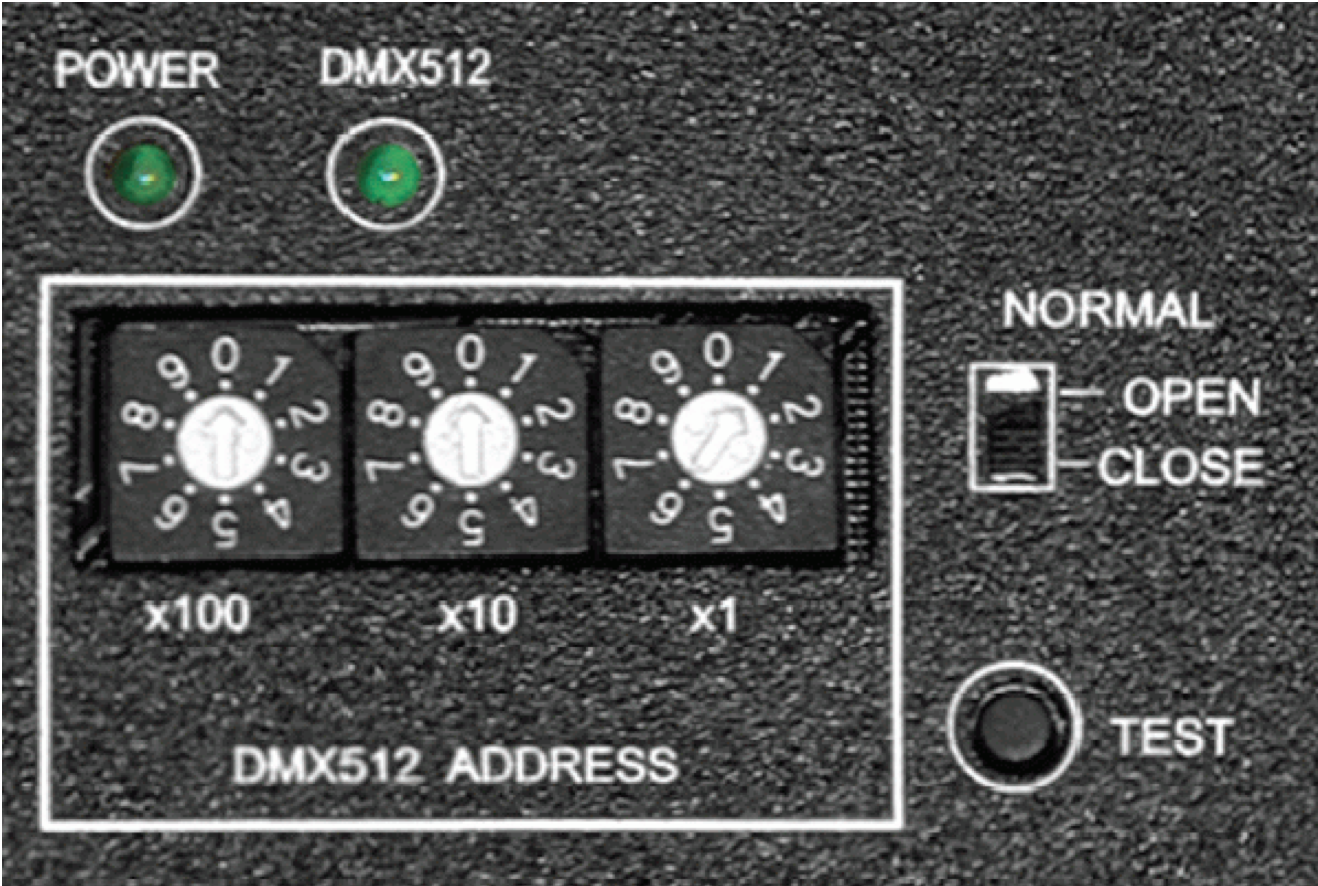
\includegraphics[height=5cm]{dial.png}
\caption{Addressing dials}
\label{fig:dial}

\end{center}
\end{figure*}

These three dials each represent hundreds, tens and units respectively. So setting an address of 159 would be a simple case of:
\begin{itemize}
\item	Turn the first dial to 1
\item	Turn the second dial to 5
\item	Turn the third dial to 9
\end{itemize}
This kind of addressing is used a lot with effects fixtures, older fixtures and dimmers.


\end{itemize}

\subsection{Rigging}

\begin{figure*}[h]
\begin{center}

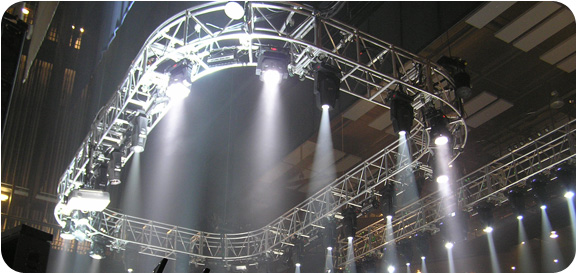
\includegraphics[height=5cm]{rigging.jpg}
\caption{A truss rig}
\label{fig:rig}

\end{center}
\end{figure*}

As you may have noticed, most lights are hung overhead from metal scaffolding poles and metal frames, which are called truss. These structures, and the process of building and suspending them, is rigging.

If you think something looks unsafe or insecure, then tell a member of Senior Crew or one of your managers immediately and we’ll sort it out.

\subsubsection{Rigging Basics}
Rigging heavy objects above people’s heads is a potentially dangerous process with huge consequences if not done correctly. In your day to day work as EUSA crew, you will not be called upon to do excessive quantities of rigging, however we will show you how to rig, hang and focus a lantern as part of your training. 

\begin{figure*}[h]
\begin{center}

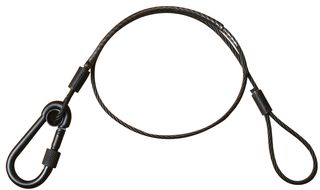
\includegraphics[height=5cm]{bond.jpg}
\caption{They call me Bond, Safety Bond}
\label{fig:bond}

\end{center}
\end{figure*}

Here are some golden rules of rigging.
\begin{itemize}
\item DO NOT exceed the Safe Working Load of any rigging, be it scaff, truss or garden hanging basket.
\item	DO make sure that everything that is hung is hanging in the manner it was designed to hang. Don’t put a shackle on sideways, don’t hang a speaker by its handles.
\item	DO make sure everything has an appropriate safety bond (Figure \ref{fig:bond}). 
\item	DO seek assistance immediately if there is anything at all to do with rigging that you’re unsure or unhappy about.

\end{itemize}

\subsubsection{Safe Working Load/Uniformly Distributed Load}
A Safe Working Load (SWL) or Uniformly Distributed Load (UDL) is the maximum amount of weight you can safely place on a particular structure. Any significant distributed or point loads need to be assessed, and may require sign-off by an engineer or qualified rigger. In most cases, we wouldn’t expect to hang enough fixtures to get anywhere near the SWL or UDL of a structure, but if you’re at all unsure, please contact the office, who will assess the load.

For example, in the Debating Hall each of the chain motors has a SWL of 400kg. Thus, the maximum amount of weight that can be suspended from each motor is 400kg. Obviously you would need to be hanging many fixtures before reaching this limit, but it’s important to also allow for the weight of the cabling!

Another example is the Pleasance Theatre lighting bars. Each bar has a UDL of 180kg, meaning that they’re rated to support up to 180kg distributed reasonably evenly along the entire bar. This limit could quite easily be reached with a larger theatre show. (For example 10 Source 4s and 4 large moving heads. This is pretty over-the-top but within the realm of possibility.)

\subsubsection{Hanging a fixture}
Below is the correct procedure for hanging a fixture, to ensure that it is safely hung and set up for focussing later on. Some of this won’t apply for moving lights.
\begin{enumerate}
\item	Place the hook clamp on the bar and tighten to secure the fixture. Please don’t overtighten, as this will damage soft aluminium truss!
\item	Attach the safety bond.
\item	Point the light in the rough direction it will be focussed and tighten the yoke bolts, both the hook clamp and tilt set.
\item	Open the barndoors / shutters to just beyond the light beam.
\item	Open the lenses to as wide as possible.
\item	Plug in power and DMX as necessary.
\item	Tape all cable neatly in place! Remember to leave enough slack cable to focus later on.
\end{enumerate}

\subsubsection{Focussing a fixture}

Obviously the way in which a light is being used will affect how it’s focussed. But there is a general approach we take to achieve the look we want:

\begin{enumerate}
\item	With the beam as wide and sharp as possible, physically point the light at the part of the stage you want to light.
\item	Carefully zoom the light to be just larger than the area you want to light.
\item	Carefully soften the focus as you need it.
\item	Bring the barndoors / shutters in to mark the area you want. Pay attention to the rotation of the barndoors, make sure the long shutters are rotated to mask the light that is most obvious to the audience.
\item	Add in any gel necessary.
\end{enumerate}


\section{AV}
\label{av}
\textbf{AV} generally refers to the display of visual content through some sort of large screen or projection. PowerPoint presentations at conferences, film nights -- many events will include some component of AV.

Many of our venues have installed AV systems, which will include some or all of the components listed below. 

\begin{itemize}
\item \textbf{Projectors}, the quintessential AV component. Come in various sizes which normally correspond with their brightness and functionality. Most projectors will include some control for focus and zoom, with some including more advanced features such as lens shift.

Keystone allows the shape of the projected image to be corrected to ensure that all sides of the image are parallel. Basic projectors will include only vertical keystone, whereas more advanced units may also include horizontal or multi point keystone (allowing each corner to be positioned individually). Note that using keystone should be used as a last resort fix for unavoidable poor positioning, and the best image quality will be achieved by placing the projector correctly.

\item Within the organisation, \textbf{LCD Displays} tend to be installed on walls, however we own a pair of LCDs on wheeled stands that can useful for small events or where a projected image would be washed out by the ambient lighting.

\item \textbf{Switchers} are generally basic units that take multiple inputs and allow the user to choose one to route to a single output. However, more complicated units called \textbf{Matrix Switchers} exist that allow any input to be routed to any of its outputs. We have matrix switchers in Library Bar and Sports Bar, and while these generally take care of themselves, it is worth knowing these exist!

\item \textbf{Scalers} are processing units used to scale the resolution of inputs to one that is supported by the output device. Generally these also include some ability to switch between inputs in a seamless fashion, and feature both analogue and digital inputs and outputs. A scaler is installed in the Debating Hall AV rack.
\end{itemize}

\subsection{Connectors}

Connectors can generally be split into \textbf{digital} and \textbf{analogue} signal types. 

\subsubsection{Digital}
\begin{itemize}
\item \textbf{HDMI: } a connector that you're likely familiar with from home use. HDMI is generally available on modern laptops, or can be passively (that is 'without power') converted to from connectors such as Mini DisplayPort or Thunderbolt. It is notable that HDMI cannot carry analogue signals, and thus if being connected to an analogue output source will require 'active' (powered) conversion. Some of our newer projectors support HDMI input.
\end{itemize}

\subsubsection{Analogue}
\begin{itemize}
\item \textbf{VGA: } Until recently (when HDMI became the default on laptops and the like), the main way to connect your computer to a projector. This connector carries analogue signal only, and thus can degrade more seriously over distance. We have converter boxes that allow this signal to be sent over CAT5/6 cable installed in our venues.
\item \textbf{Composite: } The general output format from standard definition video gear -- found on DVD players, cameras and the like. Uses an RCA connector to carry the video, and normally an additional pair to carry stereo audio.
\item \textbf{Component: } May be found on more professional video gear. Features a separate cable for three different 'components' of the video signal. It is not used sufficiently to justify further detail here, but some of our projectors will accept signals provided in this format.
\end{itemize}


%\begin{figure}[h]
%\begin{center}
%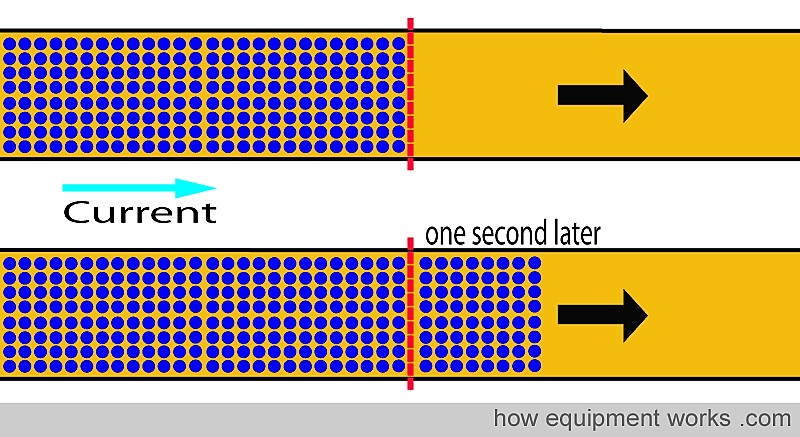
\includegraphics[width=9cm]{one-second-current2.jpg}
%\caption{The electrons passing through a cross section of the wire.}
%
%\label{fig:one-second-current}
%\end{center}
%\end{figure}

 



\end{document}

%----------------------------------------------------------------------------------------
%	ARTICLE CONTENTS
%----------------------------------------------------------------------------------------